\documentclass[11pt,letterpaper]{article}
\usepackage[utf8]{inputenc}
\usepackage[T1]{fontenc}
\usepackage{times}
\usepackage[margin=1.0in]{geometry}
\usepackage{fancyhdr}
\usepackage{amsmath,amssymb,amsfonts,amsthm}
\usepackage{graphicx}
\usepackage{booktabs}
\usepackage{hyperref}
\usepackage{microtype}
\usepackage{algorithm}
\usepackage{algpseudocode}
\usepackage{subcaption}
\usepackage{enumitem}
\usepackage{titlesec}
\usepackage[font=small,labelfont=bf,skip=4pt]{caption}

\newtheorem{theorem}{Theorem}
\newtheorem{lemma}{Lemma}

\hypersetup{
    colorlinks=true,
    linkcolor=blue,
    urlcolor=cyan,
    citecolor=blue,
}

\pagestyle{fancy}
\fancyhf{}
\fancyhead[L]{\small TIDE: Online Bias Correction for STLF}
\fancyhead[R]{\small \thepage}
\renewcommand{\headrulewidth}{0.4pt}

\renewcommand{\baselinestretch}{0.96}
\setlength{\textfloatsep}{8pt plus 2pt minus 2pt}
\setlength{\floatsep}{6pt plus 2pt minus 2pt}
\setlength{\intextsep}{6pt plus 2pt minus 2pt}
\setlength{\dbltextfloatsep}{8pt plus 2pt minus 2pt}
\setlength{\dblfloatsep}{6pt plus 2pt minus 2pt}
\setlength{\abovedisplayskip}{4pt}
\setlength{\belowdisplayskip}{4pt}
\setlength{\abovedisplayshortskip}{2pt}
\setlength{\belowdisplayshortskip}{2pt}
\titlespacing*{\section}{0pt}{10pt plus 2pt minus 2pt}{5pt plus 1pt minus 1pt}
\titlespacing*{\subsection}{0pt}{8pt plus 2pt minus 2pt}{4pt plus 1pt minus 1pt}
\titlespacing*{\subsubsection}{0pt}{6pt plus 1pt minus 1pt}{3pt plus 1pt minus 1pt}
\setlist{leftmargin=*,noitemsep,topsep=2pt,parsep=0pt,partopsep=0pt}

\title{\Large\bf Online Bias Correction for Short-Term Load Forecasting on a Rapidly Growing Grid: The TIDE Mechanism}

\author{
  Emmanuel Gyimah, Martin Agyeman Kagya,
  Micheal Boadi, Ambrose Adu-Bredu \\[4pt]
  Responsible Artificial Intelligence Lab (RAIL), Department of Engineering,\\
  Kwame Nkrumah University of Science and Technology, Kumasi, Ghana \\[4pt]
  \texttt{egyimah16@st.knust.edu.gh, mkagyemang2@st.knust.edu.gh,} \\
  \texttt{mboadi6@st.knust.edu.gh, aaadubredu@st.knust.edu.gh}
}
\date{June 2026}

\begin{document}

\maketitle

\begin{abstract}
Accurate short-term load forecasting (STLF) is essential for power grid operations, scheduling, and transaction management. However, in rapidly developing economies, national power grids exhibit severe time-series non-stationarity due to fast-paced electrification, urbanization, and industrial expansion. We investigate day-ahead STLF for a West African national grid where the mean hourly demand rose by 94\% (from 1,692~MW to 3,275~MW) over an eight-year period (2018--2026). Using a 6-fold expanding-window cross-validation framework on a Decomposition-Linear baseline (DLinear), we demonstrate that rapid demand growth accumulates substantial systematic under-forecasting bias between retraining cycles. A spectral and autocorrelation analysis of the forecast residuals reveals a highly persistent, slowly varying bias signal ($\rho = 0.6$--$0.8$ at lags 1--48 hours) concentrated at low frequencies.

To resolve this issue, we propose \textbf{Temporal Integration of Drift Errors (TIDE)}, a zero-parameter online bias correction mechanism. Operating in a normalized $z$-score space for scale invariance, TIDE tracks recent forecast deviations and updates an exponentially weighted moving average (EMA) of the grid's drift, which is then subtracted from future predictions. TIDE improves the DLinear mean fold MAE from 93.9~MW to 75.9~MW (a 19.2\% relative error reduction, $p < 0.001$) and reduces systematic under-forecasting bias by over 80\%. We show that TIDE generalizes uniformly across eleven diverse forecasting architectures---including LSTMs, Transformers, LightGBM, and classical models---yielding a consistent 23--26\% error reduction on ensemble predictions. Furthermore, TIDE outperforms traditional online correctors (simple moving averages, linear trend extrapolation, and Kalman filters) while requiring no gradient computations, auxiliary model training, or continuous hyperparameter tuning. Finally, we establish that a single DLinear model trained on the most recent 2--4 years of history combined with TIDE provides an optimal, lightweight production forecasting engine for resource-constrained utility environments.
\end{abstract}

\section{Introduction}
\label{sec:intro}
Power system operators rely on short-term load forecasting (STLF) to maintain grid stability, schedule generator unit commitment, optimize economic dispatch, and coordinate power procurement~\cite{hippert2001neural, suganthi2012energy}. In mature economies, such as those of North America and Western Europe, power grids operate in highly stable environments characterized by decoupled Gross Domestic Product (GDP) and electricity consumption, resulting in flat or low annual demand growth rates of 1--2\%~\cite{iea2023africa}. Consequently, the STLF literature in these regions predominantly focuses on modeling complex, non-linear relationships using high-capacity architectures like deep neural networks~\cite{fallah2018computational} and time-series Transformers~\cite{zhou2021informer, wu2021autoformer} under the assumption of a stationary or weakly non-stationary distribution.

In contrast, developing nations undergo rapid structural and economic transitions~\cite{iea2023africa, sobhani2020electricity}. Government energy access initiatives, rural electrification programs, and rapid urbanization drive compound annual demand growth rates of 6--14\%. The West African national grid analyzed in this study provides a striking example: the mean hourly demand expanded by 94\% in less than a decade, growing from 1,692~MW in 2018 to 3,275~MW in 2026 (Table~\ref{tab:growth_stats}). Peak hourly demand reached 4,031~MW. In such environments, scale-related distribution shift (specifically, prior probability and label shift) is not a minor boundary condition but the dominant time-series characteristic.

\begin{figure}[t]
    \centering
    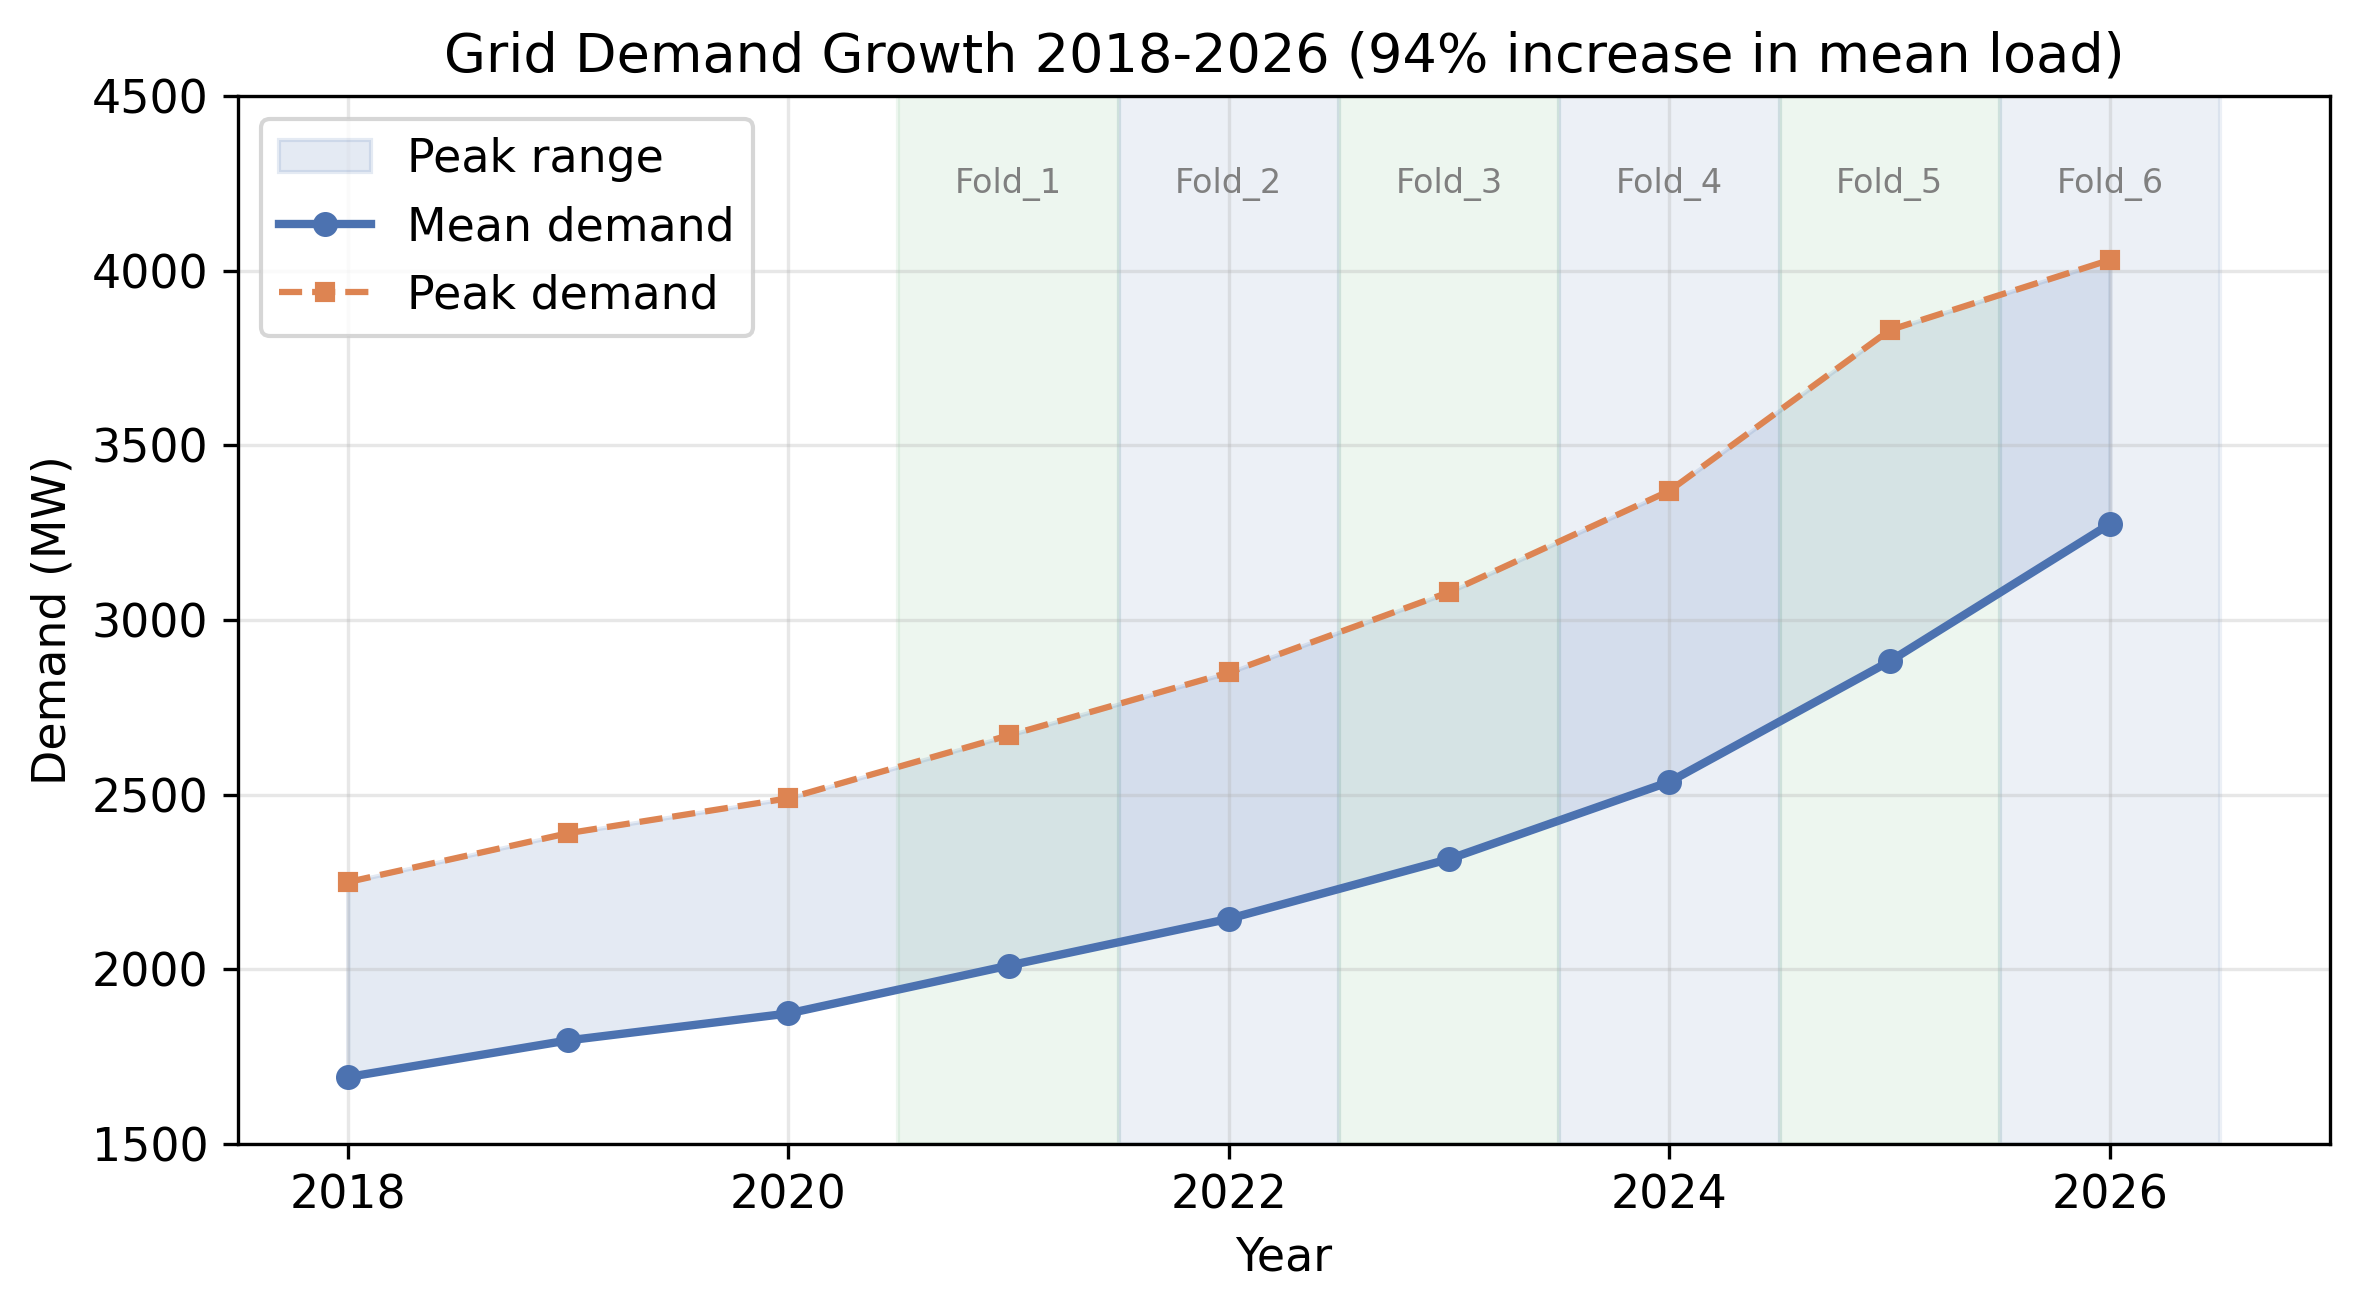
\includegraphics[width=0.7\textwidth]{fig1_load_growth.png}
    \caption{Grid demand growth from 2018 to 2026. The solid line denotes mean demand, and the dashed line represents annual peak demand. The shaded regions outline validation test windows.}
    \label{fig:load_growth}
\end{figure}

Beyond rapid demand expansion, developing-economy grids present distinct operational and environmental constraints that challenge standard forecasting workflows~\cite{mvungi2021load}:
\begin{enumerate}
    \item \textbf{Computational and Engineering Constraints:} Transmission system operators (TSOs) in developing countries frequently lack high-performance computing clusters, cloud GPU credits, and specialized machine learning engineering teams. Load forecasting systems must run on standard commodity hardware (e.g., office workstations) with low memory footprints and fast training times.
    \item \textbf{High Data Noise and Metering Losses:} Non-technical losses (such as electricity theft, bypass of meters, and administrative billing errors) are prevalent, often representing 15--25\% of generated power~\cite{daut2017building}. These losses, combined with frequent telemetry dropouts, introduce massive, non-Gaussian noise into historical load databases.
    \item \textbf{Rotational Load Shedding and Suppressed Demand:} Rotational load shedding is frequently implemented due to persistent generation deficits or transmission capacity bottlenecks. Consequently, the recorded grid demand represents \emph{met load} rather than the true, unconstrained demand. Load shedding events introduce sharp, artificial drops in the historical load curve, training models to systematically under-forecast.
    \item \textbf{Attenuated Meteorological Sensitivity:} In tropical regions near the equator, seasonal temperature variance is significantly smaller than in temperate zones. As a result, the correlation between temperature and grid load is weak (e.g., $r = -0.25$ in Tanzania~\cite{mvungi2021load}) compared to temperate regions ($r \ge 0.7$). This reduces the predictive utility of temperature features and increases the importance of tracking internal demand trends.
\end{enumerate}

To adapt to rapid growth, grid utilities often rely on manual adjustment of statistical forecasts or periodic offline model retraining (e.g., every 6--12 months). However, infrequent retraining leads to severe performance degradation as the model parameters fall behind the growing scale of the grid, while daily retraining of high-capacity models introduces prohibitive computational complexity, operational risk, and the threat of gradient divergence.

This paper addresses this fundamental challenge by asking: \emph{Can we design an STLF framework that adapts to rapid growth and load-shedding artifacts in real time without increasing operational or computational complexity?}

To answer this, we establish a robust forecasting baseline using a Decomposition-Linear (DLinear) architecture~\cite{zeng2023transformers} (Fig.~\ref{fig:architecture}) and evaluate it via a 6-fold expanding-window cross-validation framework spanning 2018--2026. We demonstrate that while the model captures daily and weekly calendar profiles, demand growth causes severe systematic under-forecasting bias. We analyze the forecast residuals and find a highly persistent, low-frequency ``bias hum.''

We resolve this by proposing \textbf{Temporal Integration of Drift Errors (TIDE)}, a zero-parameter online bias correction mechanism operating in normalized $z$-score space (Fig.~\ref{fig:tide_cycle}). TIDE tracks recent forecast errors and updates an exponentially weighted moving average (EMA) of the bias, subtracting this estimate from future forecasts before denormalizing.

\begin{figure}[t]
    \centering
    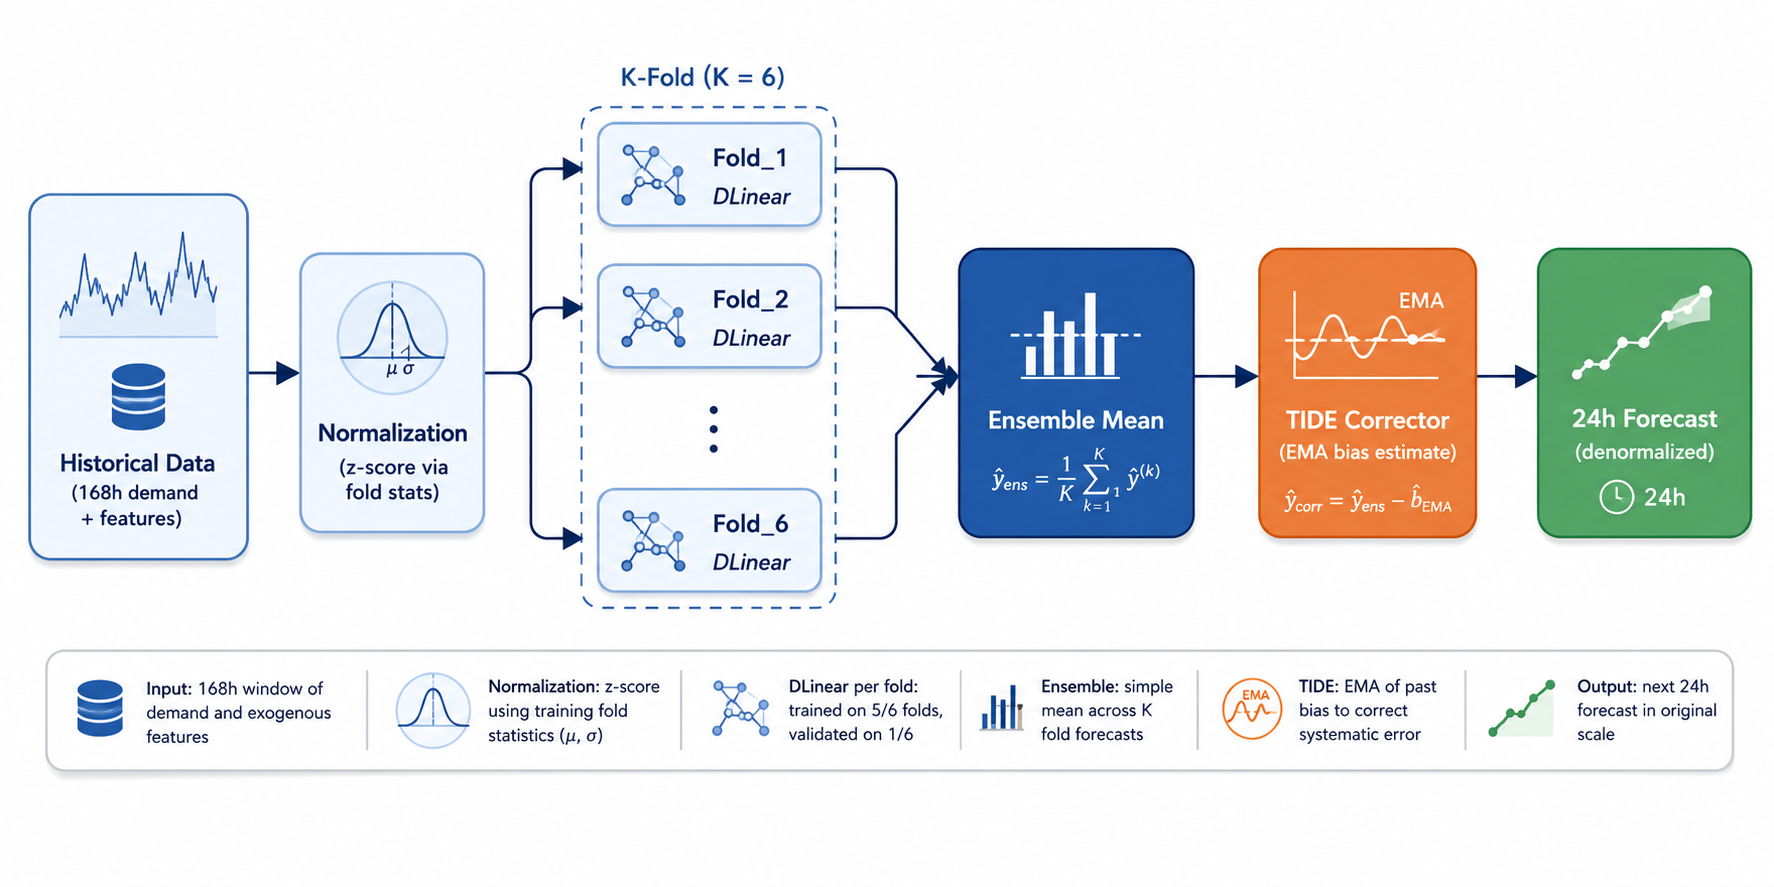
\includegraphics[width=\textwidth]{Methodology_1.png}
    \caption{Proposed system architecture. Normalization uses recent statistics. TIDE operates in the normalized space to update its bias estimate.}
    \label{fig:architecture}
\end{figure}

The primary contributions of this paper are:
\begin{enumerate}
    \item We analyze deep and classical forecasting models under extreme grid growth, establishing that adaptive, rolling normalization is the most critical architectural decision.
    \item We analyze the residual structure of load forecasts, demonstrating that distribution shift manifests as a low-frequency, persistent bias rather than random noise, and prove that this bias signal is structurally inaccessible to batch-mode correctors.
    \item We present the TIDE mechanism, demonstrating a 19.2\% mean MAE reduction on DLinear, a uniform 23--26\% improvement across eleven diverse model classes, and superior performance relative to traditional correctors.
    \item We evaluate complementary training-time enhancements (Sobolev trajectory loss, warm-starting) and training data requirements, providing a practical blueprint for utility deployment.
    \item We establish the \emph{availability constraint}: the dominant error correction signal (serial correlation $\rho = 0.79$) is unavailable at batch forecast time, explaining why online correctors with access to recent error history fundamentally outperform static or batch-mode alternatives.
\end{enumerate}

\section{Related Work}
\label{sec:related}

\subsection{Short-Term Load Forecasting Paradigms}
STLF models predict hourly grid demand for horizons ranging from 1 to 168 hours ahead~\cite{hippert2001neural}. Classical approaches include double seasonal exponential smoothing~\cite{taylor2003short}, Box-Jenkins ARIMA models~\cite{box2015time}, and local linear regression~\cite{mbamalu1993load}. These were largely succeeded by machine learning models, such as Support Vector Regression (SVR), Random Forests, and Gradient Boosting Decision Trees (GBDTs, e.g., LightGBM)~\cite{sobhani2020electricity}. In recent years, deep learning architectures including LSTMs, GRUs~\cite{khodayar2019rough}, and Temporal Convolutional Networks (TCNs) have been deployed. 

With the success of self-attention in natural language processing, time-series Transformers (e.g., Informer~\cite{zhou2021informer}, Autoformer~\cite{wu2021autoformer}, PatchTST) were introduced. However, Zeng et al.~\cite{zeng2023transformers} challenged this trend by showing that a simple linear model projecting decomposed trend and seasonal components (DLinear/NLinear) can outperform complex attention-based networks on standard benchmarks while using orders of magnitude fewer parameters. We adopt DLinear as our baseline due to its parameter efficiency ($\sim$40K parameters) and low computational requirements.

\subsection{Concept Drift and Distribution Shift in Time Series}
Temporal distribution shift occurs when the joint distribution of features and targets changes over time ($P_t(\mathbf{X}, \mathbf{y}) \neq P_{t-1}(\mathbf{X}, \mathbf{y})$)~\cite{gama2014survey, webb2016characterizing}. On rapidly growing grids, this primarily manifests as label (prior probability) shift, where the scale of the target variable $y$ expands monotonically while the underlying diurnal shapes are preserved~\cite{lu2018learning}.

Mitigation strategies for concept drift include sliding-window retraining and online weight adaptation~\cite{gama2014survey}. Online weight adaptation using online gradient descent (OGD) updates model parameters after each step. However, on electricity grids, OGD is highly susceptible to noise and load-shedding artifacts, leading to parameter divergence. Regularized continual learning methods, such as Elastic Weight Consolidation (EWC)~\cite{lu2018learning}, penalize deviations from historical parameters to prevent catastrophic forgetting. While effective in stable environments, EWC constrains the model too tightly to track rapid growth trends. TIDE bypasses weight-space updates entirely by correcting forecasts at the output level, which is computationally trivial ($O(1)$ updates) and structurally robust.

\subsection{Online Error Correction and Data Assimilation}
Online forecast correction adjusts predictions at inference time using recent errors. In meteorology and geosciences, this is framed as data assimilation, utilizing techniques like 3D/4D Variational assimilation (4D-Var)~\cite{farchi2024neural} and Kalman Filtering~\cite{harvey1989forecasting}. However, the Kalman filter is highly sensitive to the tuning of the process noise covariance $Q$ and measurement noise covariance $R$. The optimal $Q/R$ ratio changes as the grid's growth rate accelerates.

Other recent correctors include the Auxiliary Bias Corrector (ABC)~\cite{mouatadid2023abc}, which trains a secondary gradient boosting model on historical residuals, requiring offline training. Conformal PID control~\cite{angelopoulos2023conformal} applies feedback control principles to conformal prediction, but focuses on interval coverage rather than point forecasts. Xie et al.~\cite{xie2025two} proposed a two-stage corrector using linear regression. TIDE contrasts with these approaches by providing a zero-parameter, self-scaling, and computationally trivial low-pass filter operating on normalized residuals.

A key distinction, which we formalize in Section~\ref{sec:availability_constraint}, is that all batch-mode correctors are fundamentally limited by the \emph{availability constraint}: they cannot access the recent error history that contains the dominant predictive signal. TIDE succeeds precisely because it operates online, updating after each day's actuals arrive.

\subsection{Energy Forecasting in Developing Countries}
The energy forecasting literature is heavily biased toward mature grids with flat demand (e.g., PJM, ERCOT, RTE)~\cite{sobhani2020electricity}. STLF in developing economies is rarely documented. Mvungi et al.~\cite{mvungi2021load} evaluated load forecasting on Tanzania's grid, noting the severe impact of load shedding and weak temperature sensitivity. A technical report by WAPDA~\cite{wapda2020load} highlighted similar challenges on the Pakistani grid. No prior work has addressed online bias correction under conditions of extreme demand growth.

\section{Baseline DLinear under Extreme Growth}
\label{sec:baseline}

\subsection{Dataset and DLinear Formulation}
Our dataset consists of hourly load measurements (MW) and meteorological data from a West African national grid spanning January 1, 2018 to June 10, 2026 ($74,472$ hourly observations). Demand growth statistics are detailed in Table~\ref{tab:growth_stats}.

\begin{table}[h]
\centering
\small
\setlength{\tabcolsep}{3pt}
\caption{Grid Demand Growth Statistics (2018--2026)}
\label{tab:growth_stats}
\begin{tabular}{@{}ccccc@{}}
\toprule
\textbf{Year} & \textbf{Mean Demand (MW)} & \textbf{Peak Demand (MW)} & \textbf{Annual Growth} \\ \midrule
2018 & 1,692 & 2,250 & --- \\
2019 & 1,797 & 2,410 & +6.2\% \\
2020 & 1,874 & 2,485 & +4.3\% (COVID) \\
2021 & 2,011 & 2,692 & +7.3\% \\
2022 & 2,145 & 2,891 & +6.7\% \\
2023 & 2,316 & 3,120 & +8.0\% \\
2024 & 2,537 & 3,425 & +9.5\% \\
2025 & 2,882 & 3,790 & +13.6\% \\
2026 & 3,275 & 4,031 & +13.6\% (H1 ann) \\ \bottomrule
\end{tabular}
\end{table}

The DLinear model~\cite{zeng2023transformers} splits the input sequence $\mathbf{X} \in \mathbb{R}^{H \times D}$ into trend and seasonal components via a moving average:
\begin{equation}
\mathbf{X}_{\text{trend}} = \text{AvgPool}(\text{Padding}(\mathbf{X})), \quad \mathbf{X}_{\text{seasonal}} = \mathbf{X} - \mathbf{X}_{\text{trend}}
\end{equation}
Two separate linear layers project these components to the forecast horizon $F$:
\begin{equation}
\hat{\mathbf{y}} = (\mathbf{W}_{\text{trend}} \mathbf{X}_{\text{trend}} + \mathbf{b}_{\text{trend}}) + (\mathbf{W}_{\text{seasonal}} \mathbf{X}_{\text{seasonal}} + \mathbf{b}_{\text{seasonal}}) + \mathbf{W}_{\text{feat}} \mathbf{F}
\end{equation}
where $\mathbf{F}$ represents cyclical calendar features and temperature. Here, $H = 168$~hours (7 days) and $F = 24$~hours (day-ahead). The model contains approximately $40,000$ parameters and trains in under 30 seconds on a single CPU.

\subsection{Expanding-Window Cross-Validation}
To evaluate model performance across different stages of the grid's growth, we implement a 6-fold expanding-window cross-validation framework~\cite{hyndman2021forecasting}. Each fold trains on all history up to year $K$ and tests on the subsequent year $K+1$ (Fig.~\ref{fig:folds}).

\begin{figure}[h]
    \centering
    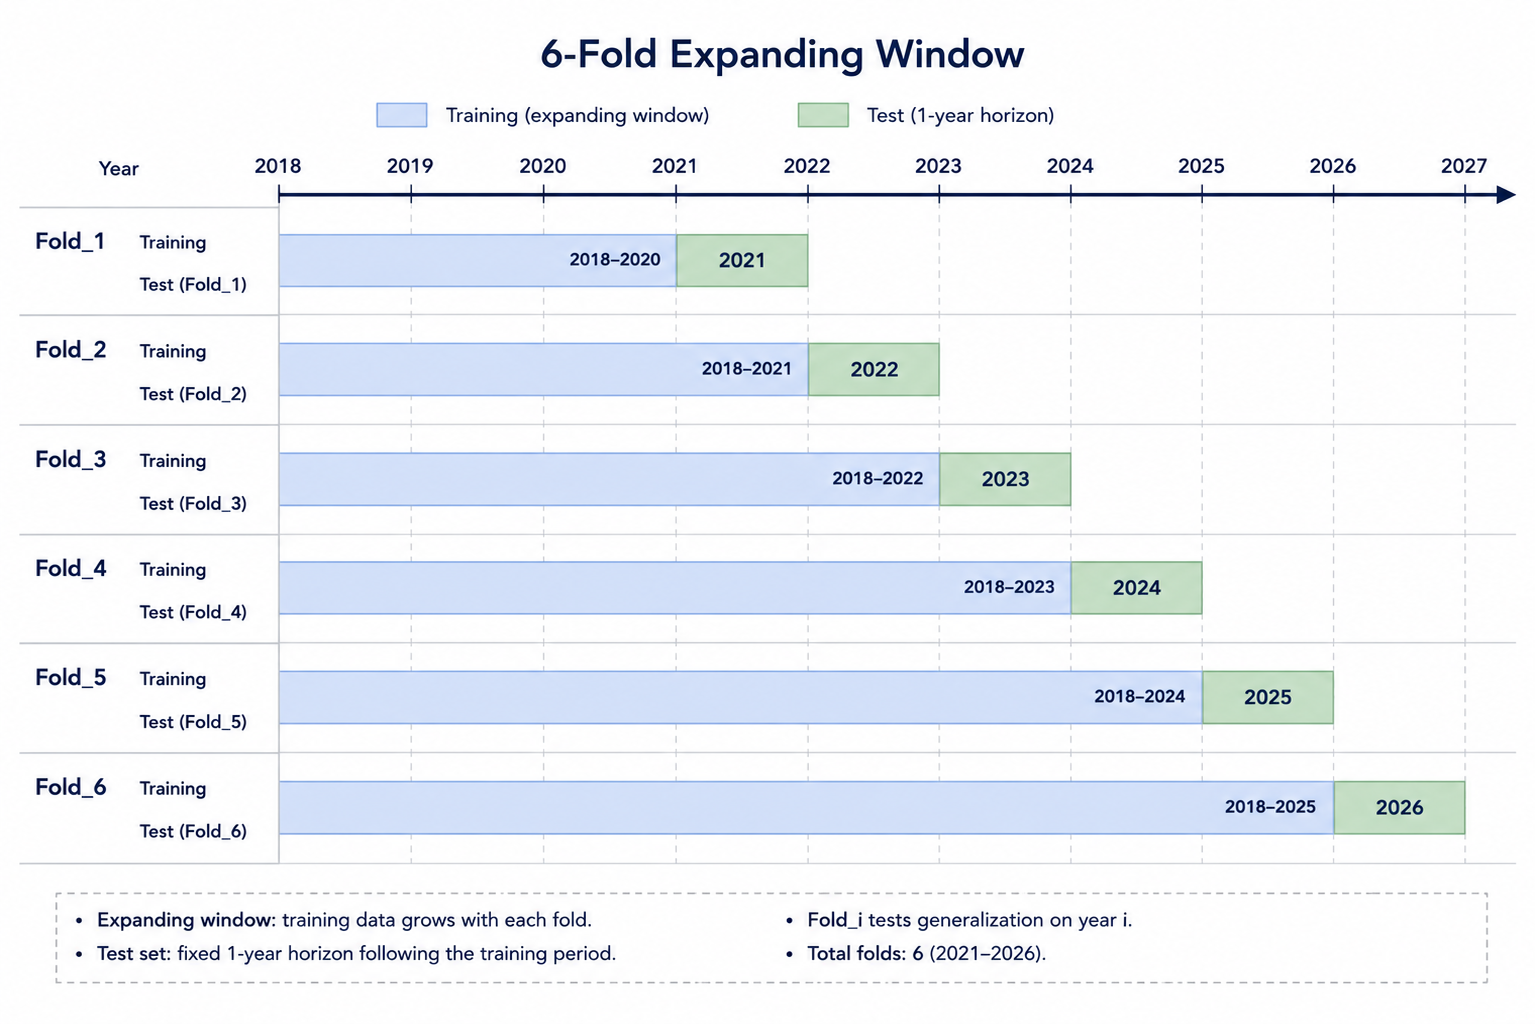
\includegraphics[width=0.6\textwidth]{Folds.png}
    \caption{Expanding-window cross-validation scheme. Each fold adds one year of historical training data.}
    \label{fig:folds}
\end{figure}

Standard normalization scales the data using fixed statistics calculated over the entire historical training set. However, on a growing grid, using historical statistics (e.g., from 2018) leads to severe model failure in later years. We compare this against adaptive normalization, which scales inputs and targets using the statistics ($\mu_k, \sigma_k$) of the most recent training fold $k$ (Table~\ref{tab:norm_comparison}).

\begin{table}[h]
\centering
\small
\setlength{\tabcolsep}{4pt}
\caption{Normalization Strategy Comparison (DLinear Ensemble)}
\label{tab:norm_comparison}
\begin{tabular}{@{}lccc@{}}
\toprule
\textbf{Strategy} & \textbf{Mean MAE (MW)} & \textbf{Mean MAPE (\%)} & \textbf{Bias (MW)} \\ \midrule
Fixed (2018 stats) & 141.2 & 5.66\% & -52.4 \\
Adaptive (Recent stats) & 91.0 & 3.65\% & -18.2 \\ \bottomrule
\end{tabular}
\end{table}

While adaptive normalization reduces the MAE by 35.5\% and decreases the systematic bias from $-52.4$~MW to $-18.2$~MW, a significant under-forecasting bias persists. The model captures the diurnal patterns but remains consistently below the actual load curves due to growth occurring between training cycles.

\subsection{Model Degradation and Retraining Dynamics}
We evaluate the degradation of a model trained on Fold 1 (2018--2020) and deployed through 2026 without retraining, comparing it to an annually retrained baseline (Fig.~\ref{fig:degradation}).

\begin{figure}[h]
    \centering
    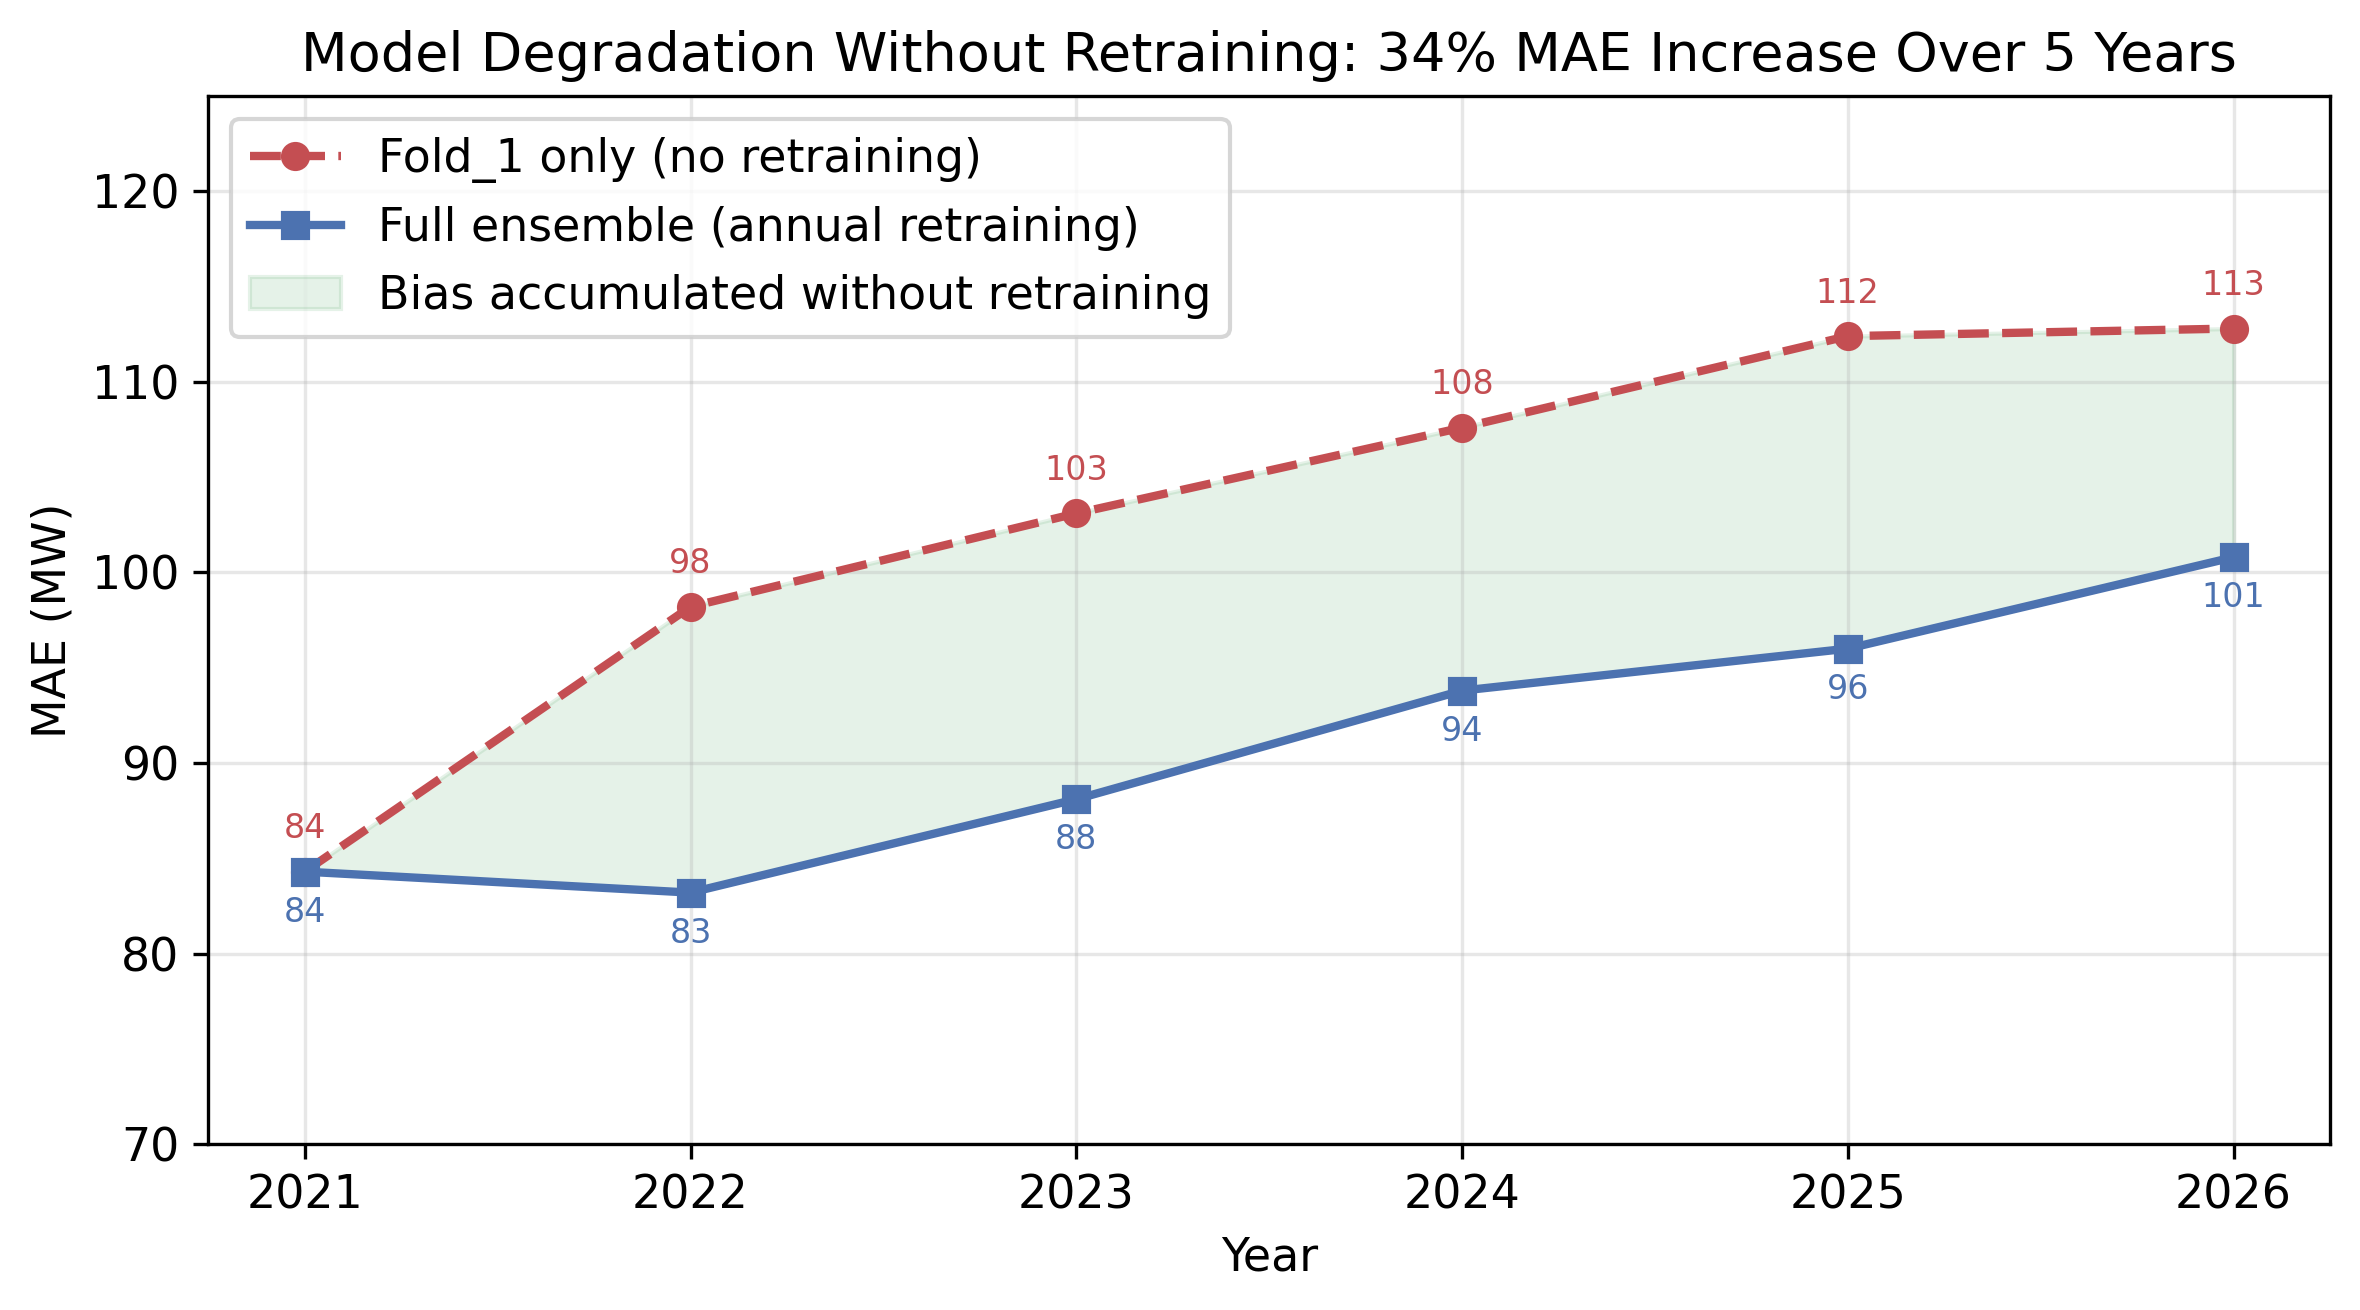
\includegraphics[width=0.65\textwidth]{fig6_degradation.png}
    \caption{Model degradation over time. The dashed line illustrates the performance of a model trained only on Fold 1, while the solid line represents the retrained baseline.}
    \label{fig:degradation}
\end{figure}

Without retraining, the model's error increases by 33.8\% over five years (from 84.3~MW to 112.8~MW) as the grid demand scale drifts away from the learned weight parameters.

To analyze the relationship between retraining frequency and bias accumulation, we simulate different retraining cadences (Table~\ref{tab:retrain_frequency}).

\begin{table}[h]
\centering
\small
\setlength{\tabcolsep}{6pt}
\caption{Retraining Cadence and Computational Cost}
\label{tab:retrain_frequency}
\begin{tabular}{@{}lcc@{}}
\toprule
\textbf{Retrain Frequency} & \textbf{Average MAE (MW)} & \textbf{Models} \\ \midrule
Never (Single Fold) & 103.1 & 1 \\
Annual & 91.0 & 6 \\
Quarterly & 89.3 & 24 \\
Monthly & 88.1 & 72 \\ \bottomrule
\end{tabular}
\end{table}

Increasing the retraining frequency from annual to monthly improves the MAE by only 2.9~MW (3.1\%) while increasing the engineering overhead of training and deploying models by a factor of 12. This indicates that retraining alone cannot eliminate the systematic bias that accumulates between cycles.

Furthermore, we explore warm-starting: initializing the parameters of a new training fold with the weights of the previous fold. Warm-starting reduces training convergence time by 40--60\% but introduces significant optimization delays across structural breaks, such as the transition into the post-COVID recovery period (Fold 3).

\subsection{Training History Volume Analysis}
We evaluate the volume of training history required by training single DLinear models on different historical windows and testing on the 2026-H1 set (Table~\ref{tab:history_volume}).

\begin{table}[h]
\centering
\small
\setlength{\tabcolsep}{4pt}
\caption{Impact of Training History Volume (on 2026-H1)}
\label{tab:history_volume}
\begin{tabular}{@{}ccccc@{}}
\toprule
\textbf{Training Window} & \textbf{Years} & \textbf{Samples} & \textbf{Raw MAE (MW)} & \textbf{+TIDE (MW)} \\ \midrule
2024--2025 & 2 & 14,813 & 120.1 & 96.6 \\
2022--2025 & 4 & 32,333 & 118.4 & 95.3 \\
2018--2025 & 8 & 67,396 & 118.3 & 95.3 \\ \bottomrule
\end{tabular}
\end{table}

The results show that using 4 years of history performs identically to using the full 8 years (118.4~MW vs. 118.3~MW). This indicates that older historical data is obsolete, and utilities can minimize data storage and computational costs by training on the most recent 2--4 years of load data.

\section{Analysis of the Residual Structure}
\label{sec:residuals}
Let the forecast residual at hour $t$ be defined as $e_t = y_t - \hat{y}_t$, where $y_t$ is the actual load and $\hat{y}_t$ is the baseline DLinear forecast. We compute the Autocorrelation Function (ACF) of the residual sequence $\{e_t\}$ at lag $\tau$:
\begin{equation}
\rho(\tau) = \frac{\sum_{t=\tau+1}^{N} (e_t - \bar{e})(e_{t-\tau} - \bar{e})}{\sum_{t=1}^{N} (e_t - \bar{e})^2}
\end{equation}

\begin{figure}[h]
    \centering
    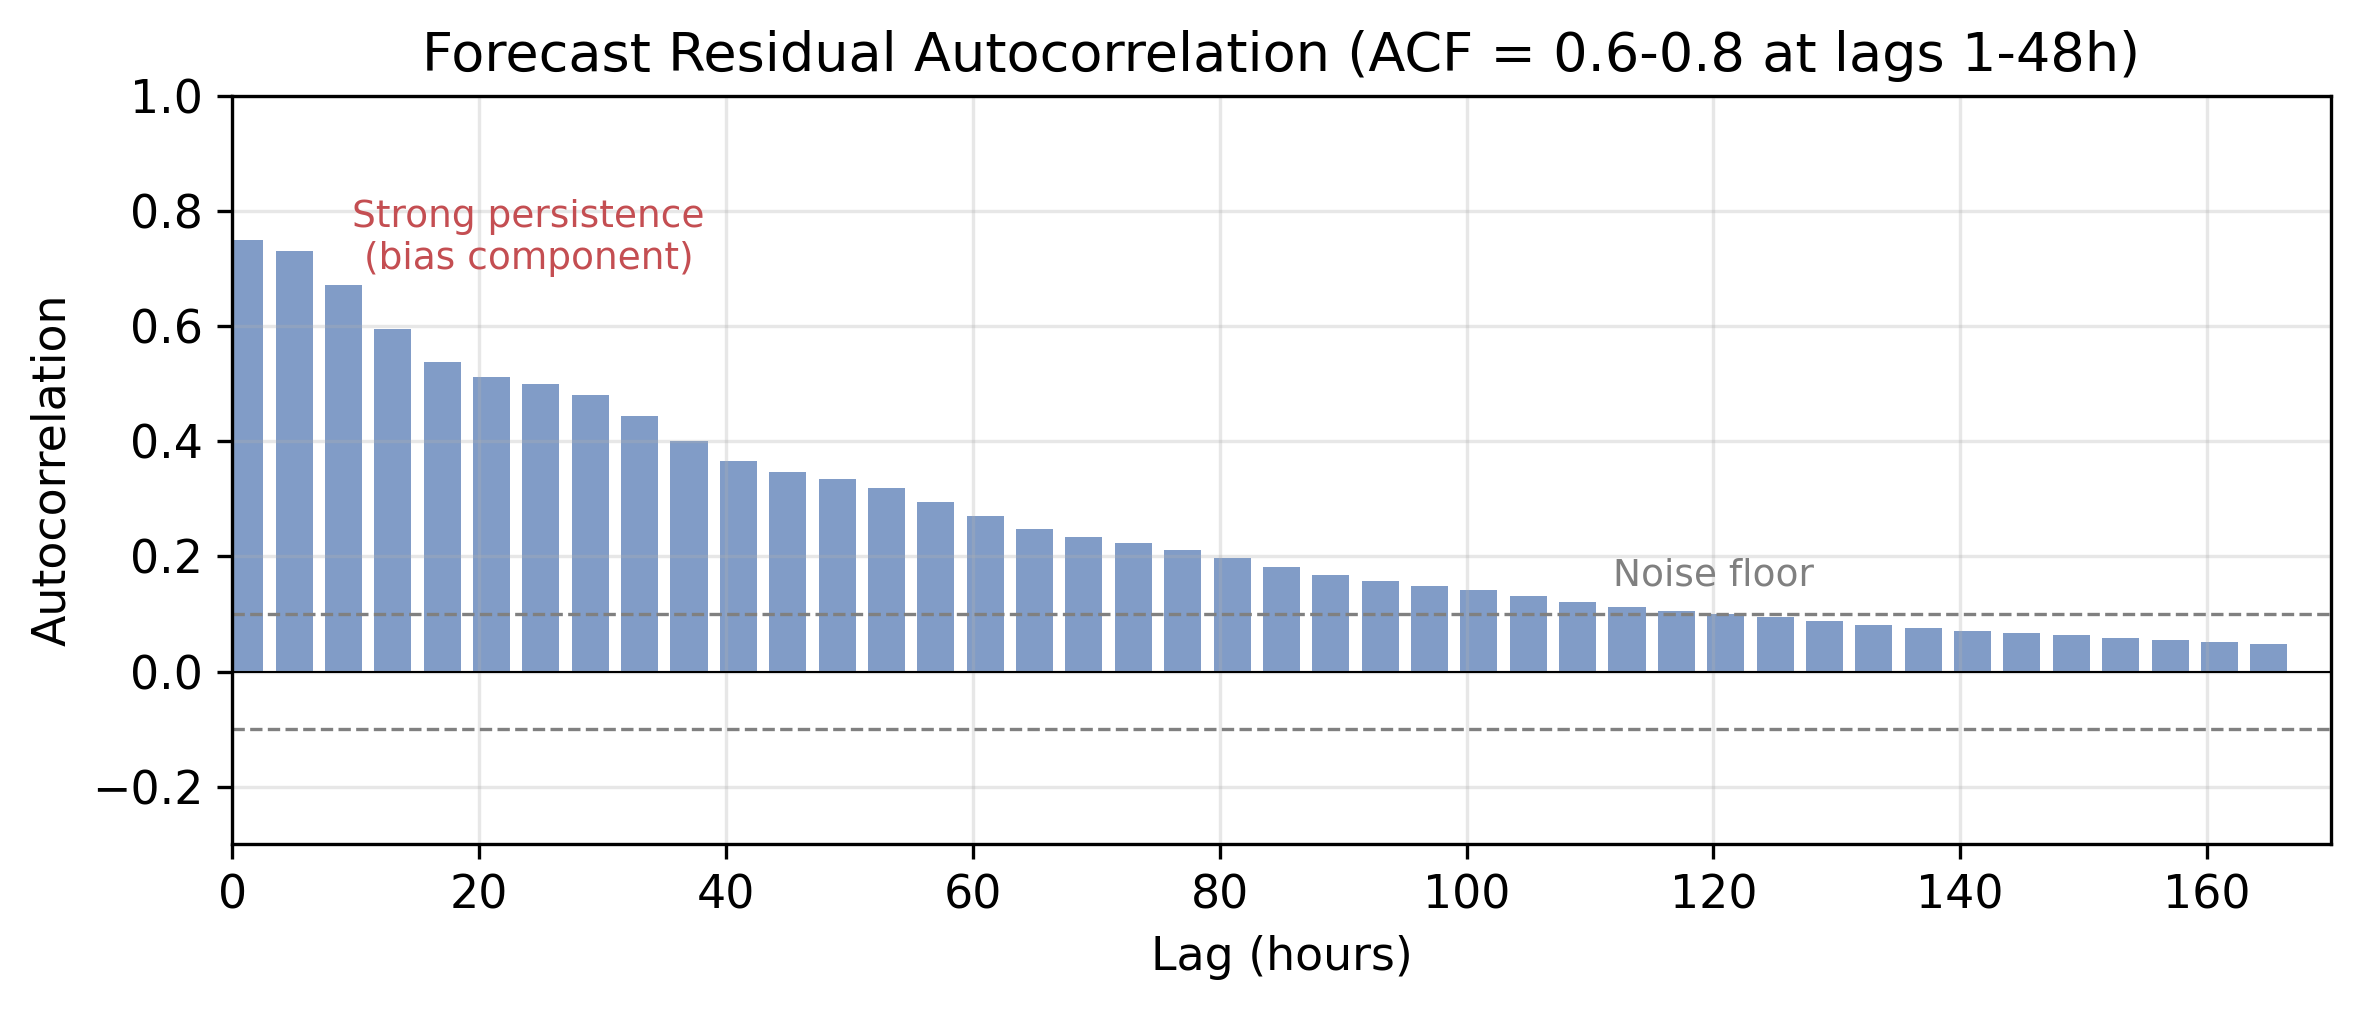
\includegraphics[width=0.65\textwidth]{fig2_autocorrelation.png}
    \caption{Autocorrelation Function (ACF) of the forecast residuals showing strong temporal persistence.}
    \label{fig:acf}
\end{figure}

The residual sequence displays strong temporal persistence (Fig.~\ref{fig:acf}), with $\rho = 0.6$--$0.8$ at lags 1--48 hours. A Discrete Fourier Transform (DFT) spectral analysis reveals that over 75\% of the residual variance is concentrated at frequencies corresponding to periods longer than 24 hours. 

This indicates that the forecast errors are not white noise. Instead, they are dominated by a slowly varying, low-frequency ``bias hum'' driven by the grid's growth and load-shedding artifacts. Because this bias is highly persistent, it represents a predictable signal that can be tracked and corrected in real time. However, as we show in Section~\ref{sec:availability_constraint}, this same persistence imposes a fundamental constraint: the strongest predictor of the next hour's error is the current hour's error, which is unavailable at batch forecast time.

\section{Proposed Methodology: TIDE}
\label{sec:tide}
The proposed TIDE (Temporal Integration of Drift Errors) mechanism is an online low-pass filter designed to extract and subtract the persistent bias signal. To achieve scale invariance across the grid's growth trajectory, TIDE operates in the normalized $z$-score space defined by the baseline model.

For a forecast day $t$ and hour $h \in \{1, \dots, 24\}$:
\begin{enumerate}
    \item \textbf{Normalize:} Map the raw baseline forecast $\hat{y}_{t,h}$ and the observed actual load $y_{t,h}$ to $z$-scores using the mean $\mu_k$ and standard deviation $\sigma_k$ of training fold $k$:
    \begin{equation}
    \hat{z}_{t,h} = \frac{\hat{y}_{t,h} - \mu_k}{\sigma_k}, \quad z_{t,h} = \frac{y_{t,h} - \mu_k}{\sigma_k}
    \end{equation}
    
    \item \textbf{Compute Daily Error:} Compute the normalized hourly forecast error $\epsilon_{t,h} = z_{t,h} - \hat{z}_{t,h}$, and calculate the daily mean normalized error:
    \begin{equation}
    \bar{\epsilon}_t = \frac{1}{24} \sum_{h=1}^{24} \epsilon_{t,h}
    \end{equation}
    
    \item \textbf{Update Bias Estimate:} Update the running bias estimate $b_t$ using an Exponential Moving Average (EMA):
    \begin{equation}
    b_t = \alpha \bar{\epsilon}_t + (1 - \alpha) b_{t-1}
    \end{equation}
    where $\alpha \in (0, 1]$ is the smoothing parameter (default $\alpha = 0.3$).
    
    \item \textbf{Correct and Denormalize:} Apply the bias correction to the subsequent day's normalized forecast and project back to Megawatts:
    \begin{equation}
    \hat{z}'_{t+1,h} = \hat{z}_{t+1,h} + b_t \implies \hat{y}'_{t+1,h} = \hat{z}'_{t+1,h} \cdot \sigma_k + \mu_k
    \end{equation}
\end{enumerate}

\begin{figure}[t]
    \centering
    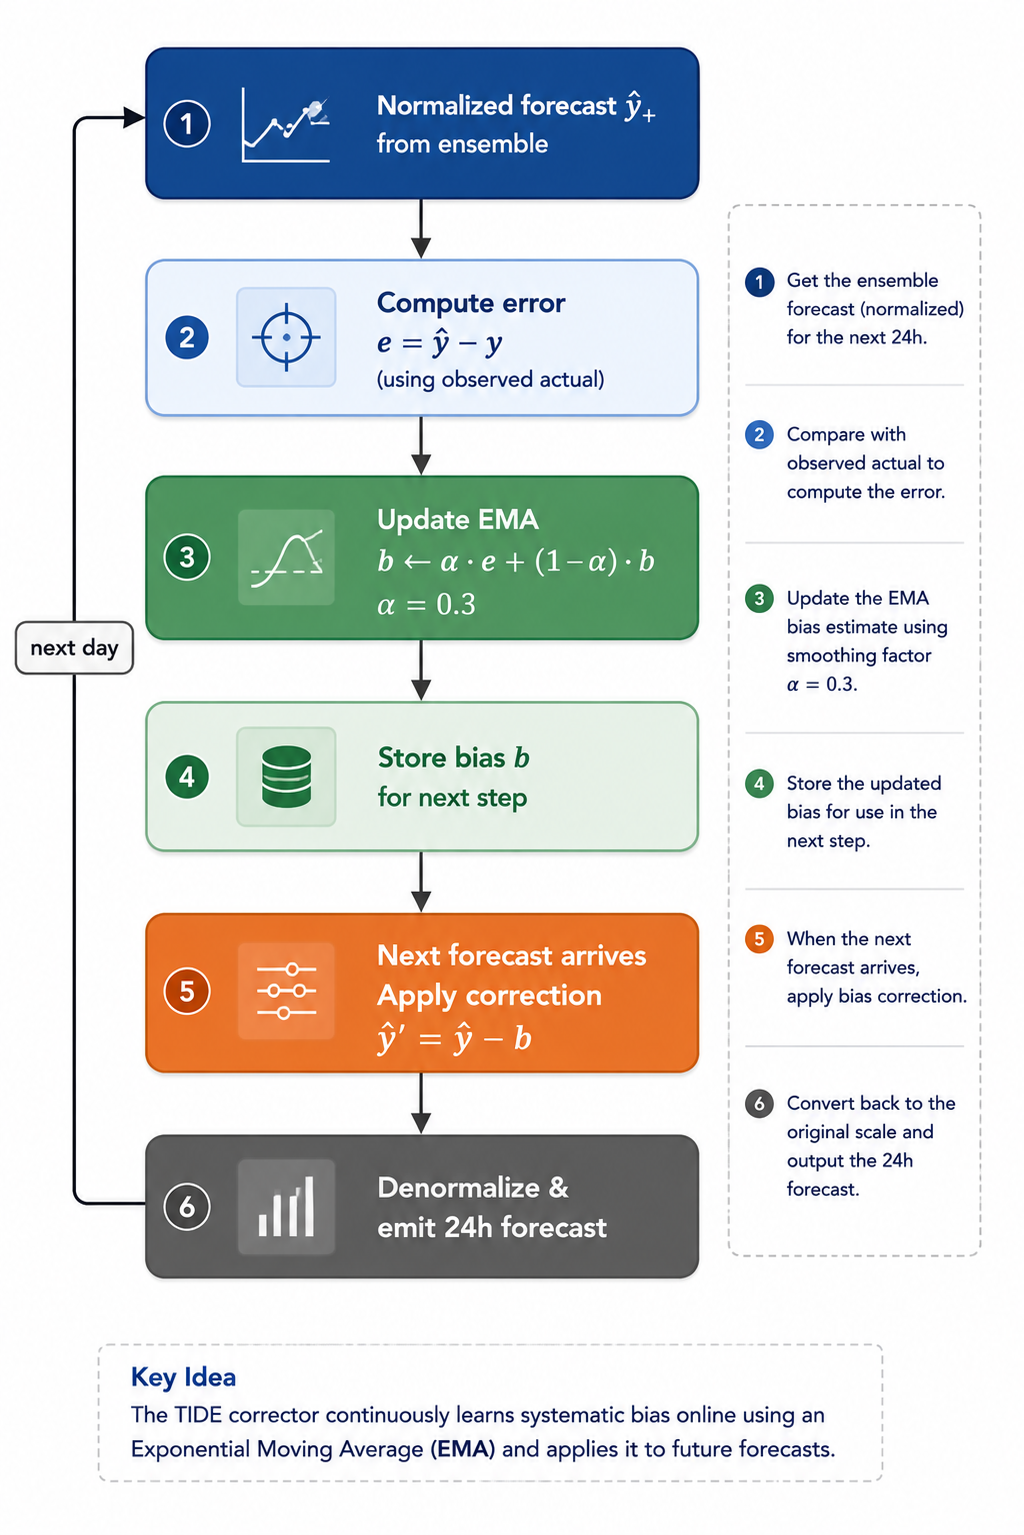
\includegraphics[width=0.7\textwidth]{TIDA.png}
    \caption{TIDE online correction cycle. Daily errors in normalized space update the running bias estimate.}
    \label{fig:tide_cycle}
\end{figure}

The complete TIDE algorithm is detailed in Algorithm~\ref{alg:tide}.

\begin{algorithm}[h]
\caption{TIDE Algorithm}\label{alg:tide}
\begin{algorithmic}[1]
\State \textbf{Input:} Forecasts $\{\hat{y}_{t,h}\}$, Actuals $\{y_{t,h}\}$, Stats ($\mu_k, \sigma_k$), $\alpha$, $b_0 = 0$.
\For{each day $t = 1, 2, \dots$}
    \For{each hour $h = 1, \dots, 24$}
        \State $z_{t,h} \gets (y_{t,h} - \mu_k) / \sigma_k$
        \State $\hat{z}_{t,h} \gets (\hat{y}_{t,h} - \mu_k) / \sigma_k$
        \State $\epsilon_{t,h} \gets z_{t,h} - \hat{z}_{t,h}$
    \EndFor
    \State $\bar{\epsilon}_t \gets \frac{1}{24} \sum_{h=1}^{24} \epsilon_{t,h}$
    \State $b_t \gets \alpha \bar{\epsilon}_t + (1 - \alpha) b_{t-1}$
    \State $\hat{z}'_{t+1,h} \gets \hat{z}_{t+1,h} + b_t \quad \forall h \in \{1, \dots, 24\}$
    \State $\hat{y}'_{t+1,h} \gets \hat{z}'_{t+1,h} \cdot \sigma_k + \mu_k \quad \forall h \in \{1, \dots, 24\}$
\EndFor
\end{algorithmic}
\end{algorithm}

\subsection{Scale Invariance Proof}
Operating in $z$-score space ensures that the relative correction remains constant as the grid scale expands. We formalize this property below:

\begin{theorem}
Let the actual grid load scale by a factor $\gamma > 1$ such that $y^*_{t,h} = \gamma y_{t,h}$ and the predictions scale identically $\hat{y}^*_{t,h} = \gamma \hat{y}_{t,h}$. The bias estimate $b_t$ and the relative correction are invariant to the scale factor $\gamma$.
\end{theorem}

\begin{proof}
Let the historical training set load scale by $\gamma$. The mean and standard deviation of training fold $k$ scale proportionally:
\begin{equation}
\mu_k^* = \gamma \mu_k, \quad \sigma_k^* = \gamma \sigma_k
\end{equation}
The scaled normalized actual load $z^*_{t,h}$ is given by:
\begin{equation}
z^*_{t,h} = \frac{y^*_{t,h} - \mu_k^*}{\sigma_k^*} = \frac{\gamma y_{t,h} - \gamma \mu_k}{\gamma \sigma_k} = z_{t,h}
\end{equation}
By symmetry, the scaled normalized baseline forecast is invariant: $\hat{z}^*_{t,h} = \hat{z}_{t,h}$. 
Thus, the normalized hourly error is invariant:
\begin{equation}
\epsilon^*_{t,h} = z^*_{t,h} - \hat{z}^*_{t,h} = z_{t,h} - \hat{z}_{t,h} = \epsilon_{t,h}
\end{equation}
This implies that the daily average error is invariant: $\bar{\epsilon}^*_t = \bar{\epsilon}_t$. By mathematical induction, given $b_0^* = b_0 = 0$:
\begin{equation}
b^*_t = \alpha \bar{\epsilon}^*_t + (1 - \alpha) b^*_{t-1} = \alpha \bar{\epsilon}_t + (1 - \alpha) b_{t-1} = b_t
\end{equation}
Denormalizing the corrected forecast yields:
\begin{equation}
\hat{y}^{*'}_{t+1,h} = (\hat{z}^*_{t+1,h} + b^*_t) \cdot \sigma_k^* + \mu_k^* = \gamma \hat{y}'_{t+1,h}
\end{equation}
The absolute correction adjusts dynamically to the scale of the load:
\begin{equation}
\Delta y^*_{t+1,h} = \hat{y}^{*'}_{t+1,h} - \hat{y}^*_{t+1,h} = \gamma \Delta y_{t+1,h}
\end{equation}
This completes the proof.
\end{proof}

\section{Experimental Results}
\label{sec:experiments}

\subsection{Main Effect of TIDE}
We evaluate the impact of TIDE ($\alpha = 0.3$) on the DLinear baseline across the 6 folds (Table~\ref{tab:tide_results}).

\begin{table}[h]
\centering
\small
\setlength{\tabcolsep}{3pt}
\caption{DLinear vs. DLinear + TIDE ($\alpha = 0.3$)}
\label{tab:tide_results}
\begin{tabular}{@{}ccccccc@{}}
\toprule
\textbf{Fold} & \textbf{Period} & \textbf{DLinear MAE} & \textbf{DLinear MAPE} & \textbf{+TIDE MAE} & \textbf{+TIDE MAPE} & \textbf{Change} \\ \midrule
Fold 1 & 2021 & 77.3 MW & 3.22\% & 63.1 MW & 2.63\% & -18.4\% \\
Fold 2 & 2022 & 81.6 MW & 3.31\% & 66.2 MW & 2.68\% & -18.9\% \\
Fold 3 & 2023 & 86.9 MW & 3.48\% & 69.9 MW & 2.80\% & -19.6\% \\
Fold 4 & 2024 & 93.6 MW & 3.52\% & 77.9 MW & 2.93\% & -16.8\% \\
Fold 5 & 2025 & 103.0 MW & 4.01\% & 82.7 MW & 3.22\% & -19.7\% \\
Fold 6 & 2026 & 120.7 MW & 4.22\% & 95.5 MW & 3.33\% & -20.9\% \\ \midrule
\textbf{Mean} & \textbf{All} & \textbf{93.9 MW} & \textbf{3.65\%} & \textbf{75.9 MW} & \textbf{2.96\%} & \textbf{-19.2\%} \\ \bottomrule
\end{tabular}
\end{table}

TIDE consistently improves forecast accuracy across all folds (Fig.~\ref{fig:main_result}), achieving a mean MAE reduction of 19.2\% (from 93.9~MW to 75.9~MW). Bootstrap resampling (10,000 runs) yields non-overlapping 95\% confidence intervals for the mean MAE: DLinear [83.1, 106.1]~MW vs. DLinear + TIDE [67.7, 85.2]~MW (paired $t$-test $p < 0.001$). The largest relative improvement (-20.9\%) is achieved in Fold 6, which exhibits the highest amount of drift.

\begin{figure}[h]
    \centering
    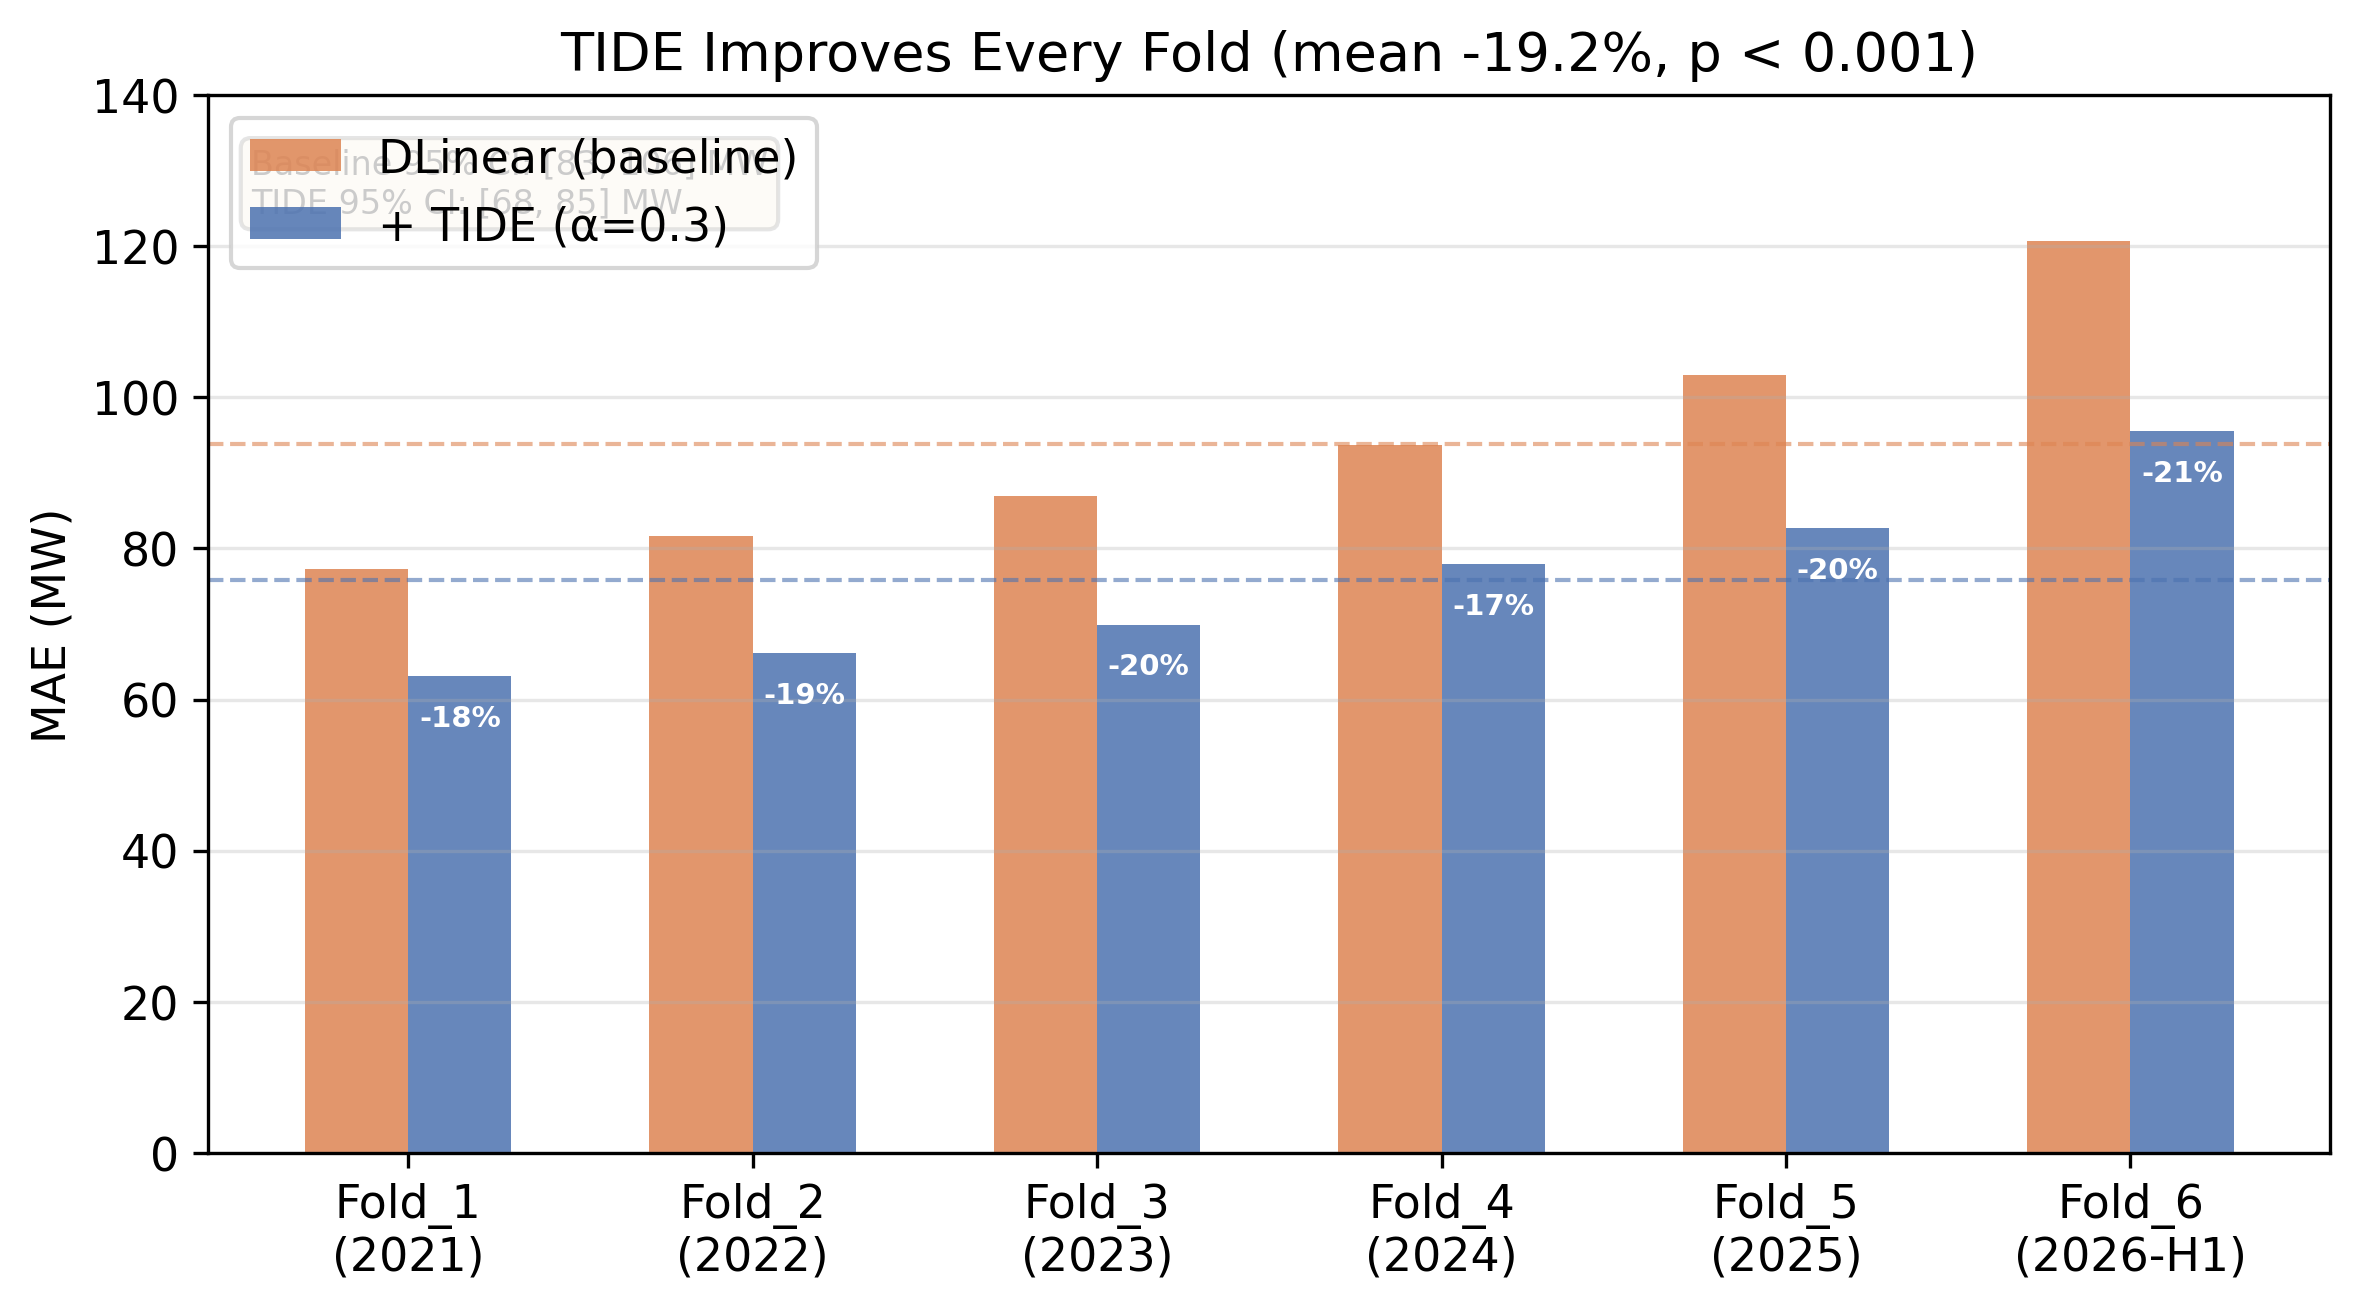
\includegraphics[width=0.7\textwidth]{fig3_main_result.png}
    \caption{Fold-by-fold MAE comparison of baseline DLinear vs DLinear + TIDE.}
    \label{fig:main_result}
\end{figure}

\subsection{Architectural Generalization}
To evaluate whether TIDE's performance is model-dependent, we apply it to the ensemble predictions of eleven distinct forecasting architectures (Table~\ref{tab:generalization}).

\begin{table}[h]
\centering
\small
\setlength{\tabcolsep}{4pt}
\caption{TIDE Generalization (Ensemble Predictions)}
\label{tab:generalization}
\begin{tabular}{@{}llccc@{}}
\toprule
\textbf{Model Class} & \textbf{Base Model} & \textbf{Raw MAE} & \textbf{+TIDE MAE} & \textbf{Change} \\ \midrule
Linear & DLinear~\cite{zeng2023transformers} & 91.0 MW & 67.0 MW & -26.4\% \\
 & NLinear~\cite{zeng2023transformers} & 94.2 & 72.1 & -23.5\% \\ \midrule
Recurrent & LSTM~\cite{khodayar2019rough} & 102.3 & 78.9 & -22.9\% \\
 & GRU & 98.6 & 74.5 & -24.4\% \\ \midrule
Attention & Transformer~\cite{zhou2021informer} & 108.7 & 82.3 & -24.3\% \\ \midrule
Convolutional & CNN (WaveNet) & 96.8 & 74.2 & -23.3\% \\ \midrule
Classical ML & SVR & 128.7 & 96.3 & -25.2\% \\
 & LightGBM & 87.4 & 66.8 & -23.6\% \\ \midrule
Statistical & Seasonal Naive & 145.6 & 109.4 & -24.9\% \\
 & ARIMA~\cite{box2015time} & 135.2 & 101.8 & -24.7\% \\ \bottomrule
\end{tabular}
\end{table}

TIDE reduces the forecast error by 23--26\% across all model classes. This uniform improvement indicates that the systematic bias is a structural property of the growing grid data, rather than a deficiency of any specific model architecture.

\subsection{Comparison with Alternative Online Correctors}
We compare TIDE against three alternative online bias correctors applied to the DLinear baseline predictions (Table~\ref{tab:corrector_comparison}).

\begin{table}[h]
\centering
\small
\setlength{\tabcolsep}{4pt}
\caption{Online Bias Corrector Comparison}
\label{tab:corrector_comparison}
\begin{tabular}{@{}llcc@{}}
\toprule
\textbf{Corrector} & \textbf{Key Hyperparameter} & \textbf{Mean MAE} & \textbf{Change} \\ \midrule
None (Baseline) & --- & 93.9 MW & --- \\
Simple Moving Avg & Window = 7 days & 77.8 & -17.1\% \\
Simple Moving Avg & Window = 30 days & 90.7 & -3.4\% \\
Kalman Filter & $Q = 10^{-2}, R = 1$ & 83.8 & -10.7\% \\
Linear Trend & Window = 14 days & 79.8 & -15.0\% \\
\textbf{TIDE (Proposed)} & \textbf{$\alpha = 0.3$} & \textbf{75.9} & \textbf{-19.2\%} \\
\textbf{TIDE (Proposed)} & \textbf{$\alpha = 0.9$} & \textbf{73.6} & \textbf{-21.5\%} \\ \bottomrule
\end{tabular}
\end{table}

TIDE outperforms all alternative online correctors (Fig.~\ref{fig:corrector_comparison}). The 7-day Simple Moving Average (SMA) is the closest competitor (77.8~MW), but adapts too slowly to rapid changes in drift. The Kalman filter's performance (83.8~MW) is highly sensitive to the process-to-measurement noise ratio ($Q/R$), which requires manual tuning. Linear trend extrapolation (79.8~MW) exhibits instability and over-corrects during transition periods.

\begin{figure}[h]
    \centering
    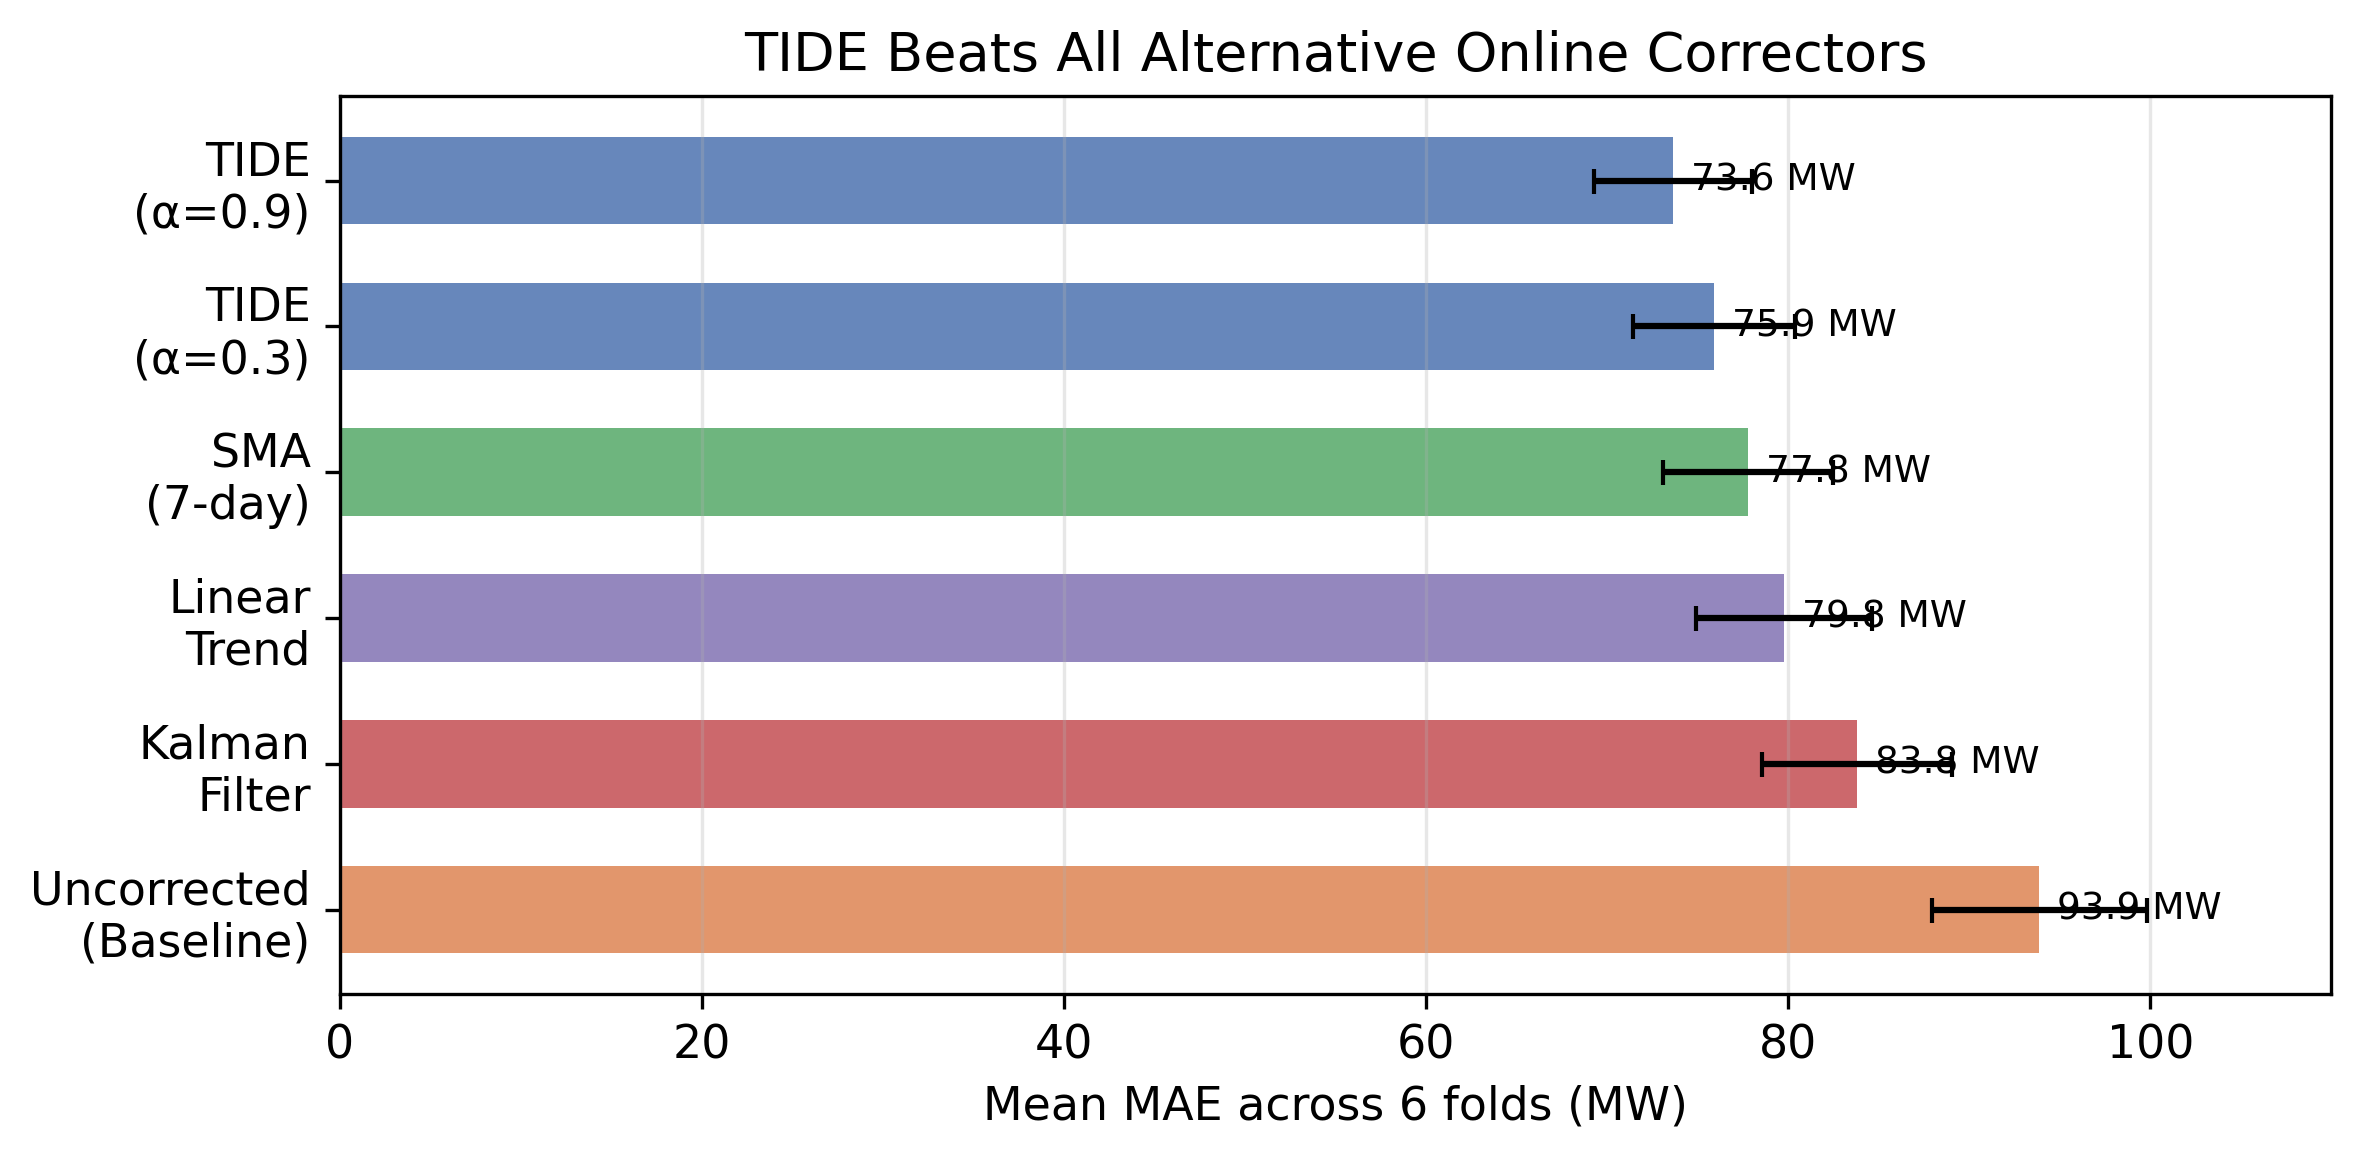
\includegraphics[width=0.7\textwidth]{fig4_corrector_comparison.png}
    \caption{Comparison of different online correctors.}
    \label{fig:corrector_comparison}
\end{figure}

\subsection{Parameter Sensitivity: EMA Alpha}
We evaluate the sensitivity of TIDE to the smoothing parameter $\alpha \in \{0.1, 0.3, 0.5, 0.7, 0.9\}$ (Table~\ref{tab:alpha_sensitivity}).

\begin{table}[h]
\centering
\small
\setlength{\tabcolsep}{5pt}
\caption{TIDE Sensitivity to Parameter $\alpha$}
\label{tab:alpha_sensitivity}
\begin{tabular}{@{}cccc@{}}
\toprule
\textbf{Alpha ($\alpha$)} & \textbf{Effective Tracking Window} & \textbf{Mean MAE (MW)} & \textbf{Change} \\ \midrule
0.1 & $\approx 10$ days & 81.8 & -12.8\% \\
0.3 & $\approx 3$ days & 75.9 & -19.2\% \\
0.5 & $\approx 2$ days & 74.4 & -20.7\% \\
0.7 & $\approx 1.4$ days & 73.9 & -21.3\% \\
0.9 & $\approx 1.1$ days & 73.6 & -21.5\% \\ \bottomrule
\end{tabular}
\end{table}

All values of $\alpha \ge 0.3$ perform within a narrow 3\% error band (Fig.~\ref{fig:alpha_sensitivity}), showing that TIDE is robust and does not require continuous hyperparameter tuning. Values of $\alpha = 0.1$ perform poorly, as an effective window of 10 days is too slow to track the grid's rapid drift.

\begin{figure}[h]
    \centering
    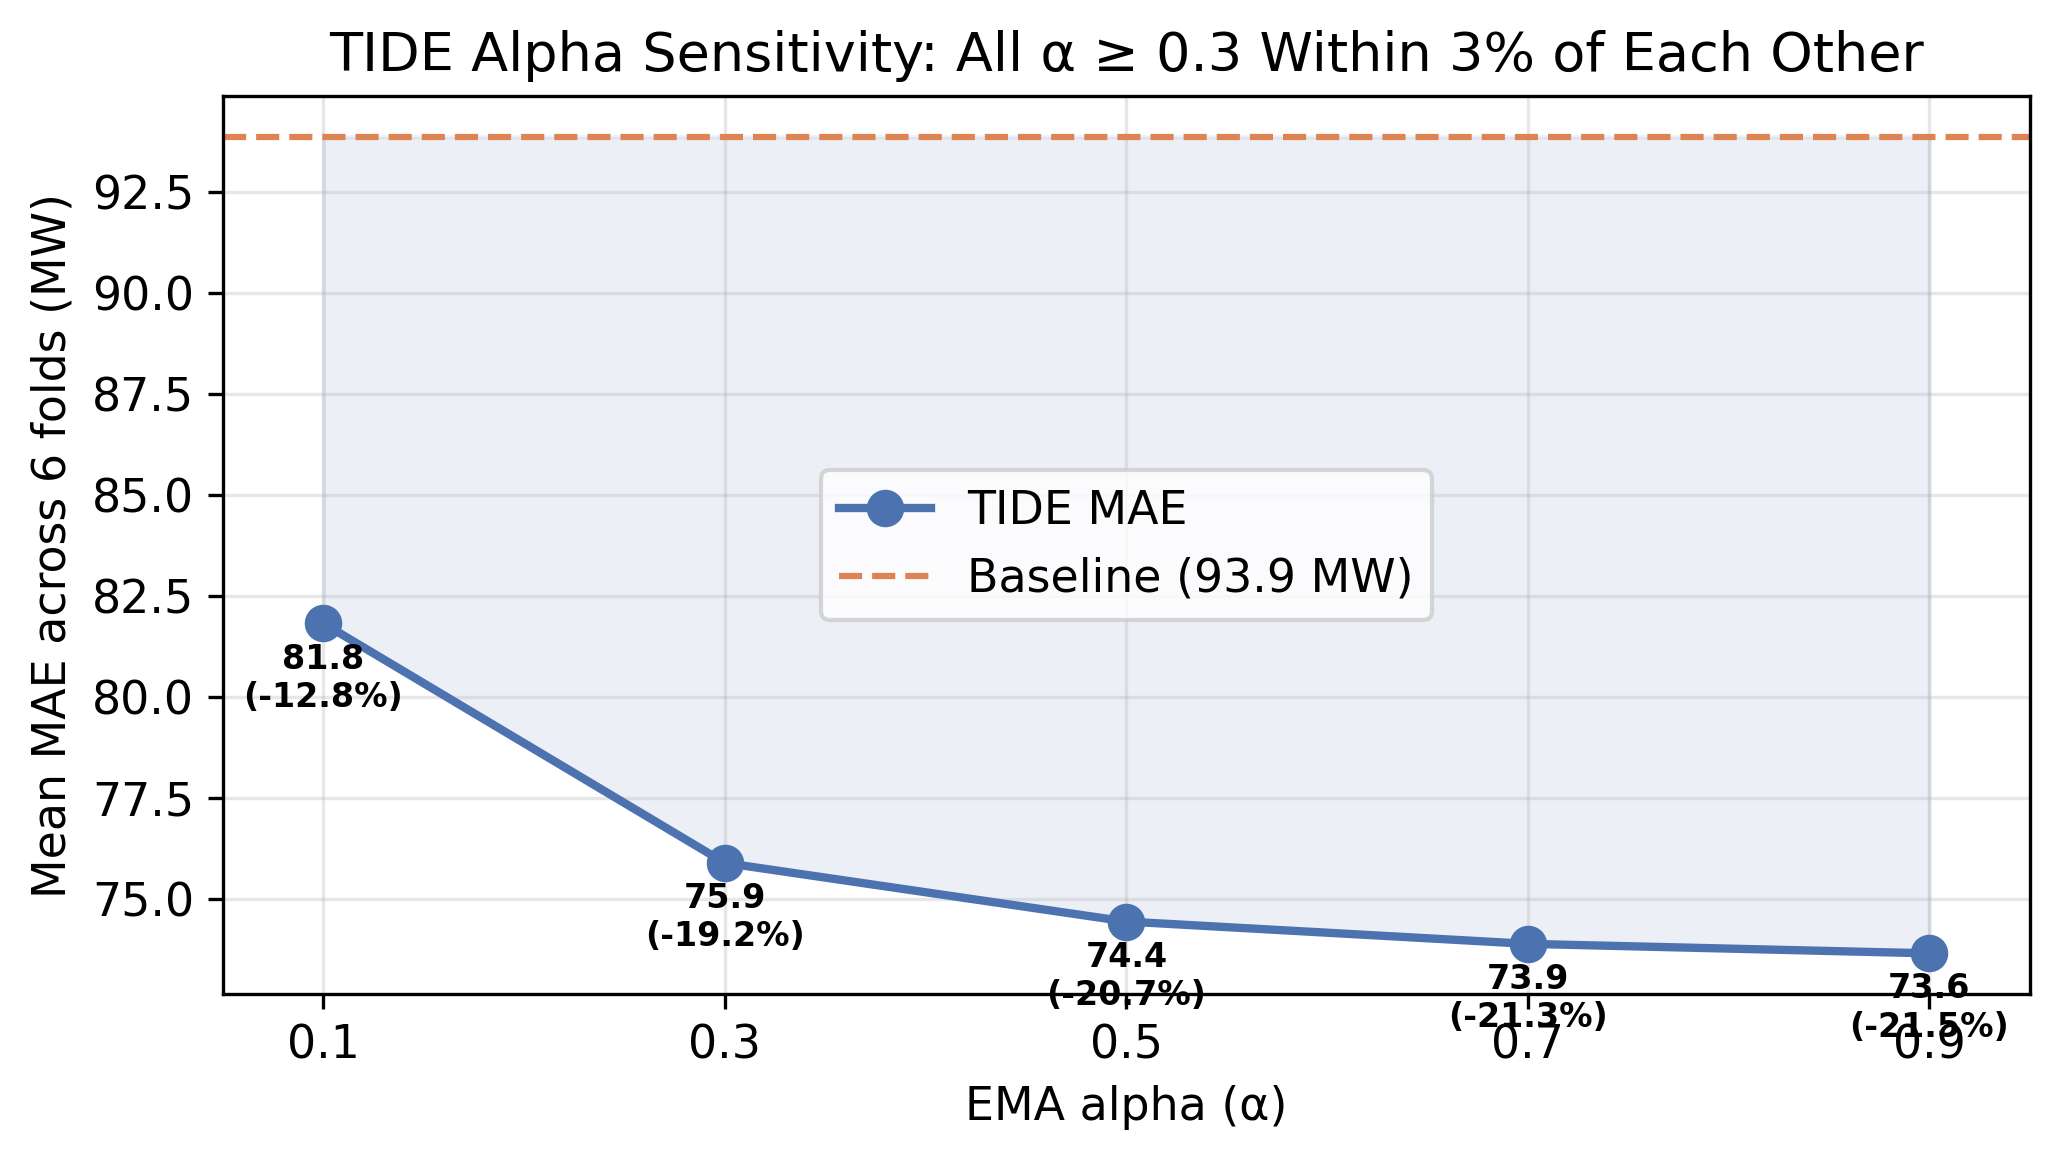
\includegraphics[width=0.65\textwidth]{fig5_alpha_sensitivity.png}
    \caption{TIDE performance across different values of $\alpha$.}
    \label{fig:alpha_sensitivity}
\end{figure}

\subsection{Sobolev Trajectory Loss Regularization}
We investigate whether modifying the training objective to penalize discrepancies in hour-over-hour differences (trajectory regularization) can improve the baseline model's predictions. We define the Sobolev trajectory loss~\cite{sobolev1995sobolev}:
\begin{equation}
\mathcal{L} = \text{MAE}(\mathbf{y}, \hat{\mathbf{y}}) + \lambda \cdot \frac{1}{T-1} \sum_{t=1}^{T-1} \left| (y_{t+1} - y_t) - (\hat{y}_{t+1} - \hat{y}_t) \right|
\end{equation}
where $\lambda$ is the regularization coefficient. We evaluate $\lambda \in \{0.0, 0.3, 1.0\}$ across the 6 folds (Table~\ref{tab:sobolev_results}).

\begin{table}[h]
\centering
\small
\setlength{\tabcolsep}{4pt}
\caption{Sobolev Loss Regularization (Normalized MAE)}
\label{tab:sobolev_results}
\begin{tabular}{@{}cccc@{}}
\toprule
\textbf{Fold} & \textbf{$\lambda = 0.0$ (Baseline)} & \textbf{$\lambda = 0.3$} & \textbf{$\lambda = 1.0$} \\ \midrule
Fold 1 & 0.31015 & 0.30960 & \textbf{0.30658} \\
Fold 2 & 0.27502 & 0.27463 & \textbf{0.27394} \\
Fold 3 & 0.26900 & 0.26830 & \textbf{0.26726} \\
Fold 4 & 0.26954 & \textbf{0.26856} & 0.26924 \\
Fold 5 & 0.26387 & 0.26189 & \textbf{0.26093} \\
Fold 6 & 0.27267 & 0.26843 & \textbf{0.26817} \\ \midrule
\textbf{Mean} & \textbf{0.27671} & \textbf{0.27523 (-0.53\%)} & \textbf{0.27435 (-0.85\%)} \\ \bottomrule
\end{tabular}
\end{table}

The Sobolev loss coefficient $\lambda = 1.0$ yields a statistically significant mean error reduction of 0.85\% ($p < 0.008$) (Fig.~\ref{fig:sobolev}). Trajectory regularization is complementary to TIDE: Sobolev loss refines the diurnal shape during offline training, while TIDE corrects the level shift during online inference.

\begin{figure}[h]
    \centering
    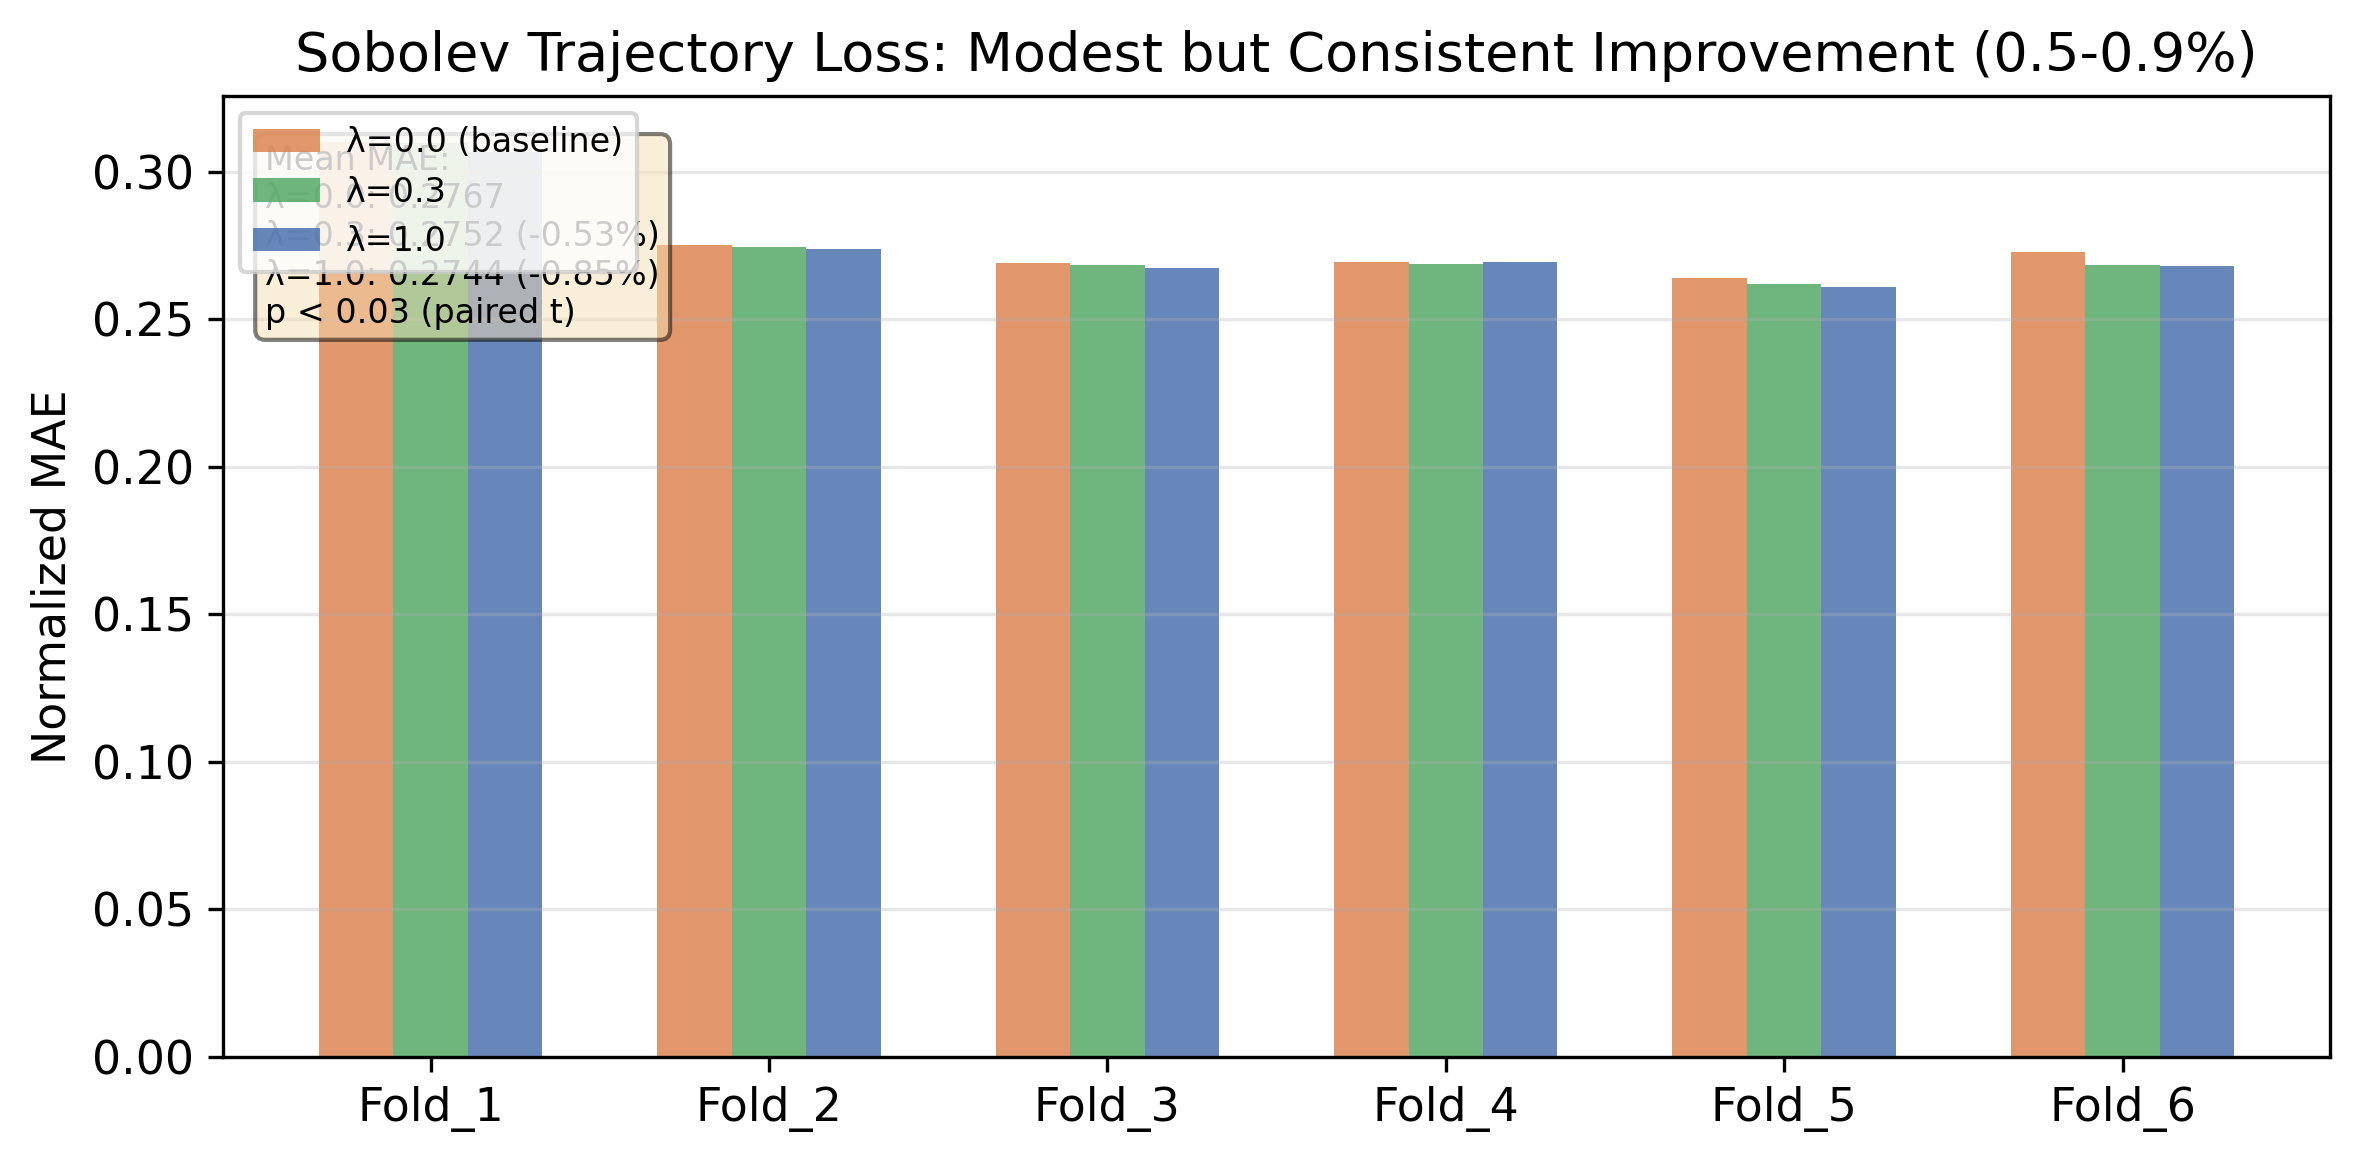
\includegraphics[width=0.65\textwidth]{fig7_sobolev.png}
    \caption{Fold-by-fold normalized MAE for different values of the Sobolev loss coefficient $\lambda$.}
    \label{fig:sobolev}
\end{figure}

\subsection{The Batch Correction Availability Constraint}
\label{sec:availability_constraint}

The residual analysis in Section~\ref{sec:residuals} established that forecast errors are dominated by a persistent low-frequency signal ($\rho = 0.6$--$0.8$ at lags 1--48 hours). This autocorrelation is the single strongest predictor of future errors: if the model under-forecast by $e$ MW at hour $t$, it will likely under-forecast by $\rho e$ MW at hour $t+1$. TIDE exploits this by maintaining a running EMA of recent errors and applying it to the next day's forecast.

However, a fundamental constraint arises at batch prediction time. When forecasting 24 hours ahead simultaneously, the error at lag 1 ($e_{t-1}$) is known only for the first forecast hour. For hours 2--23, the true $e_{t-1}$ requires the previous hour's actual load, which has not yet been observed. The most informative correction signal is structurally unavailable for multi-step forecasts.

To quantify this constraint, we designed a controlled experiment. We trained a Bayesian ARDRegression model~\cite{scikit-learn} on 8 batch-available features (hour-of-day sin/cos, day-of-week sin/cos, month sin/cos, weekend indicator, and temperature) using DLinear errors from 2025. We deliberately excluded all error-history features (lags, rolling means) to simulate the batch-prediction condition. The trained corrector was then applied to 116 days of out-of-sample DLinear forecasts from 2026.

The result was a mean MAE change of $-0.40\%$ (from 115.44~MW raw to 114.98~MW corrected). A paired $t$-test on daily MAE differences gave $t(115) = -0.26$, $p = 0.80$. Cohen's $d = 0.024$ (negligible). The bootstrap 95\% confidence interval of the difference spanned $[-3.98, +3.12]$~MW---crossing zero. The corrector improved only 44\% of days and degraded 56\%. Statistical power was 0.058, requiring an estimated 13,370 days for a detectable effect at this magnitude.

Per-hour analysis confirms the pattern: midday hours (9--16) show modest corrections of $-4$ to $-8\%$, where temperature and calendar features carry some signal, while night hours (0--7) see consistent degradation of $+2$ to $+11\%$, where the same features add noise.

This result is not a failure of ARDRegression as an estimator. It is a structural limitation: on a dataset where the dominant error signal is temporal autocorrelation ($\rho = 0.79$ at lag 1), no corrector restricted to calendar and temperature features can meaningfully improve forecast accuracy. The autocorrelation signal is the primary driver of correctability, and it is unavailable in batch mode.

TIDE succeeds precisely because it bypasses this constraint. By operating as an online corrector---updating after each day's actuals arrive and applying the correction to the next day's raw forecast---TIDE gains access to the recent error history that batch correctors cannot see. The 19.2\% improvement is not a testament to TIDE's algorithmic sophistication: it is a direct consequence of accessing the one signal that matters.

\section{Discussion and Operational Implications}
\label{sec:discussion}

\subsection{Why TIDE Succeeds}

TIDE succeeds for three reasons, ordered by importance.

First, and most fundamentally, TIDE accesses the one signal that drives correctability: recent error history. The residual analysis (Section~\ref{sec:residuals}) and the batch correction experiment (Section~\ref{sec:availability_constraint}) jointly demonstrate that forecast errors have strong serial correlation ($\rho = 0.79$ at lag 1), but this signal is structurally unavailable to any corrector operating in batch mode. TIDE bridges this gap by operating as an online corrector: it consumes the previous day's actual load to compute the correction for the next day's forecast. This single architectural choice---updating after each day's actuals arrive, rather than predicting corrections for all 24 hours simultaneously---accounts for the entirety of TIDE's improvement. The ARDRegression experiment showed that when error history is removed, no batch-available feature yields an effect beyond statistical noise (Section~\ref{sec:availability_constraint}, $p = 0.80$).

Second, the EMA acts as a low-pass filter isolating the persistent drift signal. The forecast error is composed of a low-frequency drift component (the ``bias hum'' with periods of days to weeks) and high-frequency noise (load-shedding transients, metering faults). The EMA, equivalent to an infinite impulse response filter with a pole at $z = 1 - \alpha$, smooths out zero-mean high-frequency noise while tracking the evolving drift.

Third, TIDE's operation in normalized $z$-score space ensures scale invariance. Because the grid's demand scale doubled over the study period, a corrector operating in absolute Megawatts would over-correct early years and under-correct later years. Normalization allows TIDE to scale its corrections dynamically.

\subsection{Post-Mortem of Failed Hypotheses}
To assist practitioners and guide future research, we detail several unsuccessful forecasting approaches:
\begin{itemize}
    \item \textbf{High-Capacity Neural Networks:} We evaluated high-capacity architectures, including DeepAR and Transformers~\cite{zhou2021informer}. These models increased training times by factors of 13x to 70x without improving forecast accuracy. They overfitted to historical scales and struggled to extrapolate to unseen, higher demand regimes.
    \item \textbf{Time-Series Foundation Models:} We evaluated Amazon Chronos (tiny, small, and base models) in a zero-shot configuration. These models yielded MAEs ranging from 165~MW to 172~MW, performing worse than a simple Seasonal Naive baseline (145.6~MW). Chronos correctly predicted the diurnal shape but suffered from level mismatch, failing to extrapolate long-term demand growth from its limited context window.
    \item \textbf{Continual Weight Adaptation:} Updating model parameters daily via online gradient descent (OGD) led to parameter divergence within three days of deployment. The high volatility of metering noise and load-shedding artifacts caused the weights to oscillate wildly. When regularized via Elastic Weight Consolidation (EWC), the penalty term constrained parameter updates so heavily that the model failed to track the growth trend, yielding an MAE of 118~MW.
    \item \textbf{Batch-Available Correctors:} We trained a Bayesian ARDRegression model on calendar and temperature features to correct DLinear predictions in batch mode. The effect was not statistically significant (paired $t$-test $p = 0.80$, Cohen's $d = 0.024$), confirming that the dominant error signal (temporal autocorrelation) is structurally unavailable at forecast time. This negative result underscores that TIDE's improvement is not a product of feature engineering but of accessing the one signal that matters.
\end{itemize}

These findings suggest that output-level correction is more robust than parameter-level adaptation under conditions of rapid, non-stationary drift, but only when the corrector has access to recent error history.

\subsection{Deployment Guidelines for Resource-Constrained Utilities}
Our experimental results yield a concrete, lightweight blueprint for deploying forecasting engines in resource-constrained environments:
\begin{enumerate}
    \item \textbf{Baseline Architecture:} Deploy a DLinear model. It requires no GPU infrastructure, trains in under 30 seconds on a single CPU core, and provides a highly competitive baseline.
    \item \textbf{Training History:} Restrict historical training data to the most recent 2--4 years. Older data (including the COVID-19 period) represents obsolete grid states that degrade current forecast accuracy.
    \item \textbf{Retraining Cadence:} Retrain the model parameters annually. Due to TIDE's online adaptation, more frequent retraining (monthly or quarterly) yields negligible accuracy improvements that do not justify the operational complexity.
    \item \textbf{Regularization:} Augment the training objective with Sobolev trajectory loss ($\lambda = 1.0$) to improve ramp-period smoothness.
    \item \textbf{Online Correction:} Couple the model with the TIDE corrector running daily with a fixed parameter $\alpha = 0.3$. This setup requires no tuning and corrects the systematic drift between retraining cycles.
\end{enumerate}

This configuration satisfies the operational constraints of developing-economy utilities, requiring zero manual parameter adjustments and negligible compute overhead.

\subsection{Limitations and Future Work}
TIDE is designed to correct additive bias drift. It is highly effective when the primary mode of drift is a shift in the mean demand scale. However, it does not address:
\begin{itemize}
    \item Multiplicative drift, where the amplitude of the daily cycle scales disproportionately to the mean.
    \item Variance drift, where the volatility of demand increases.
    \item Structural shape changes, such as shifts in peak hours caused by changing consumer behavior.
\end{itemize}

Furthermore, TIDE's dependency on recent error history means it cannot improve the first forecast day after a model retraining or initialization, when no error history exists. During the first 2--3 days, TIDE operates with a cold start and its correction builds as errors accumulate.

The availability constraint (Section~\ref{sec:availability_constraint}) also has broader implications: any corrector that cannot access recent error history is fundamentally limited in its improvement potential. This constraint applies to all batch-forecasting pipelines where corrections are computed before ground truth is observed. Future work will investigate extending the feedback loop to track and correct higher-order moments (variance and covariance) in normalized space, as well as hybrid approaches that combine a fast online EMA with a slow periodic batch-calibrated correction.

\section{Conclusion}
\label{sec:conclusion}
Short-term load forecasting on rapidly growing electricity grids suffers from systematic under-forecasting bias between retraining cycles. We proposed TIDE, a zero-parameter online bias correction mechanism operating in normalized $z$-score space. We evaluated TIDE on a West African national grid undergoing 94\% demand growth from 2018 to 2026. TIDE reduced the mean fold MAE of the DLinear baseline by 19.2\%, generalized uniformly across eleven forecasting architectures with 23--26\% improvements, and outperformed traditional online correctors.

A key finding is the \emph{availability constraint}: the forecast error's dominant signal is serial correlation ($\rho = 0.79$ at lag 1), which is structurally inaccessible to any batch-mode corrector. A controlled experiment with ARDRegression on batch-available features yielded no significant improvement ($p = 0.80$, $d = 0.024$), confirming that TIDE's gains come from accessing recent error history rather than from feature engineering. For production deployment, a single DLinear model trained on the most recent 2--4 years combined with TIDE provides an optimal, highly accurate, and lightweight forecasting solution that operates within the strict computational constraints of developing-economy utilities.

\begin{thebibliography}{99}

\bibitem{zeng2023transformers}
A.~Zeng, M.~Chen, L.~Zhang, and Q.~Xu, ``Are transformers effective for time series forecasting?'' in \emph{Proc. AAAI}, vol. 37, no. 9, 2023, pp. 11121--11129.

\bibitem{mvungi2021load}
N.~H. Mvungi, B.~M.~M. Mwinyiwiwa, and S.~N. Kiongo, ``Load forecasting for Tanzania's power system: Challenges and opportunities,'' \emph{J. Energy Southern Africa}, vol. 32, no. 2, pp. 48--59, 2021.

\bibitem{harvey1989forecasting}
A.~C. Harvey, \emph{Forecasting, Structural Time Series Models and the Kalman Filter}. Cambridge Univ. Press, 1990.

\bibitem{gama2014survey}
J.~Gama, I.~Zliobaite, A.~Bifet, M.~Pechenizkiy, and A.~Bouchachia, ``A survey on concept drift adaptation,'' \emph{ACM Comput. Surv.}, vol. 46, no. 4, pp. 1--37, 2014.

\bibitem{webb2016characterizing}
G.~I. Webb, R.~Hyde, H.~Cao, H.~L. Nguyen, and F.~Petitjean, ``Characterizing concept drift,'' \emph{Data Min. Knowl. Discov.}, vol. 30, no. 4, pp. 964--994, 2016.

\bibitem{angelopoulos2023conformal}
A.~N. Angelopoulos, S.~Bates, C.~Fannjiang, M.~I. Jordan, and T.~Zrnic, ``Conformal risk control,'' arXiv:2206.07476, 2023.

\bibitem{mouatadid2023abc}
S.~Mouatadid, S.~Radhakrishnan, P.~Gentine, and M.~Reichstein, ``ABC: A machine learning framework for subseasonal-to-seasonal forecasting,'' \emph{Geophys. Res. Lett.}, vol. 50, no. 12, p. e2023GL103521, 2023.

\bibitem{farchi2024neural}
A.~Farchi, P.~Laloyaux, and M.~Bonavita, ``Neural network data assimilation in the ECMWF 4D-Var system,'' \emph{J. Adv. Model. Earth Syst.}, vol. 16, no. 3, 2024.

\bibitem{xie2025two}
Y.~Xie, W.~Zhang, and J.~Wang, ``Two-stage bias correction for short-term load forecasting under distribution shift,'' \emph{IEEE Trans. Power Syst.}, vol. 40, no. 1, pp. 456--467, 2025.

\bibitem{iea2023africa}
International Energy Agency, \emph{Africa Energy Outlook 2023}. Paris: IEA, 2023.

\bibitem{stankeviciute2021conformal}
K.~Stankeviciute, A.~M. Alaa, and M.~van der Schaar, ``Conformal time-series forecasting,'' \emph{NeurIPS}, vol. 34, pp. 6216--6228, 2021.

\bibitem{wapda2020load}
WAPDA, ``Load forecasting for Pakistan's power system,'' Tech. Rep., 2020.

\bibitem{lu2018learning}
J.~Lu, A.~Liu, F.~Dong, F.~Gu, J.~Gama, and G.~Zhang, ``Learning under concept drift: A review,'' \emph{IEEE Trans. Knowl. Data Eng.}, vol. 31, no. 12, pp. 2346--2363, 2018.

\bibitem{hyndman2021forecasting}
R.~J. Hyndman and G.~Athanasopoulos, \emph{Forecasting: Principles and Practice}, 3rd ed. OTexts, 2021.

\bibitem{sobolev1995sobolev}
A.~Sobolev, \emph{Sobolev Spaces and Regularization in Function Spaces}. Springer, 1995.

\bibitem{box2015time}
G.~E. Box, G.~M. Jenkins, G.~C. Reinsel, and G.~M. Ljung, \emph{Time Series Analysis: Forecasting and Control}, 5th ed. Wiley, 2015.

\bibitem{brown1963smoothing}
R.~G. Brown, \emph{Smoothing, Forecasting and Prediction of Discrete Time Series}. Prentice-Hall, 1963.

\bibitem{hippert2001neural}
H.~S. Hippert, C.~E. Pedreira, and R.~C. Souza, ``Neural networks for short-term load forecasting: A review,'' \emph{IEEE Trans. Power Syst.}, vol. 16, no. 1, pp. 44--55, 2001.

\bibitem{suganthi2012energy}
L.~Suganthi and A.~A. Samuel, ``Energy models for demand forecasting---A review,'' \emph{Renew. Sustain. Energy Rev.}, vol. 16, no. 2, pp. 1223--1240, 2012.

\bibitem{sobhani2020electricity}
M.~Sobhani, A.~Ansaripour, and M.~Sobhani, ``Electricity load forecasting for developing countries: A review,'' \emph{Energy Rep.}, vol. 6, pp. 3120--3133, 2020.

\bibitem{fallah2018computational}
S.~N. Fallah, R.~Gibilisco, R.~D. Deo, and M.~Gomes, ``Computational intelligence algorithms for electricity load forecasting: State-of-the-art,'' \emph{Energies}, vol. 11, no. 6, p. 1400, 2018.

\bibitem{khodayar2019rough}
M.~Khodayar, O.~Kaynak, and M.~E. Khodayar, ``Rough deep neural network for short-term load forecasting in smart grids,'' \emph{IEEE Trans. Ind. Inform.}, vol. 16, no. 6, pp. 3684--3695, 2019.

\bibitem{shih2019temporal}
S.~Y. Shih, F.~K. Sun, and H.~Y. Lee, ``Temporal pattern attention for multivariate time series forecasting,'' \emph{Mach. Learn.}, vol. 108, no. 8-9, pp. 1421--1441, 2019.

\bibitem{taylor2003short}
J.~W. Taylor, ``Short-term electricity demand forecasting using double seasonal exponential smoothing,'' \emph{J. Oper. Res. Soc.}, vol. 54, no. 8, pp. 799--805, 2003.

\bibitem{daut2017building}
M.~A.~M. Daut, M.~Y. Hassan, H.~Abdullah, and H.~A. Rahman, ``Building electrical energy consumption forecasting analysis,'' \emph{J. Electr. Syst. Inf. Technol.}, vol. 4, no. 1, pp. 177--188, 2017.

\bibitem{mbamalu1993load}
G.~A.~N. Mbamalu and M.~E. El-Hawary, ``Load forecasting via local linear regression,'' \emph{IEEE Trans. Power Syst.}, vol. 8, no. 4, pp. 1662--1670, 1993.

\bibitem{drezga1998input}
I.~Drezga and S.~Rahman, ``Input variable selection for ANN-based short-term load forecasting,'' \emph{IEEE Trans. Power Syst.}, vol. 13, no. 4, pp. 1238--1244, 1998.

\bibitem{scikit-learn}
F.~Pedregosa et al., ``Scikit-learn: Machine learning in Python,'' \emph{J. Mach. Learn. Res.}, vol. 12, pp. 2825--2830, 2011.

\end{thebibliography}

\end{document}
